% ============================================================
% Chapter: Implementation of the Digital Twin Pipeline
% ============================================================
% Insert into main thesis with: % ============================================================
% Chapter: Implementation of the Digital Twin Pipeline
% ============================================================
% Insert into main thesis with: % ============================================================
% Chapter: Implementation of the Digital Twin Pipeline
% ============================================================
% Insert into main thesis with: % ============================================================
% Chapter: Implementation of the Digital Twin Pipeline
% ============================================================
% Insert into main thesis with: \input{chapter_implementation}
% Required packages in preamble:
%   \usepackage{booktabs, tabularx, listings, xcolor, graphicx,
%               hyperref, amsmath, amssymb, float, caption}
% ============================================================

\chapter{Implementation of the Physical-to-Digital Twin Pipeline}
\label{ch:implementation}

\section{Overview}
\label{sec:impl-overview}

This chapter describes the end-to-end implementation of the hydrogen plant
digital twin pipeline.
The system translates continuous sensor output from a simulated alkaline
electrolyser and hydrogen compression plant into a queryable, monitored
time-series database, and exposes the data to authenticated external
consumers through a REST API.

The pipeline follows a layered architecture, illustrated schematically in
Figure~\ref{fig:pipeline-overview}, organised around five concerns:
simulation, streaming, quality assurance, storage, and exposition.
Each layer is independently testable and replaceable.

\begin{figure}[H]
  \centering
  % Replace with actual architecture diagram
  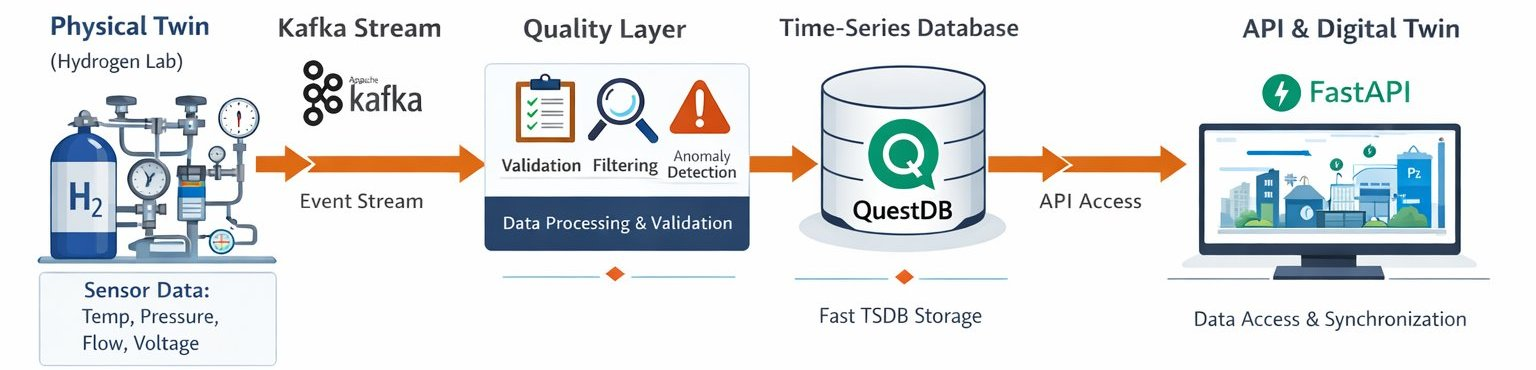
\includegraphics[width=0.95\textwidth]{images/github_internship_image_cropped.jpg}
  \caption{High-level architecture of the Physical-to-Digital Twin pipeline.
           Sensor telemetry flows left to right: simulator $\to$ Kafka $\to$
           ingestion service $\to$ QuestDB $\to$ API and monitoring.}
  \label{fig:pipeline-overview}
\end{figure}

All services are containerised and orchestrated with Docker Compose.
The implementation language is Python~3.11 throughout, with
FastAPI~\cite{fastapi} for the API layer,
confluent-kafka~\cite{confluentkafka} for Kafka connectivity,
PyJWT and bcrypt for authentication, and
structlog~\cite{structlog} for structured logging.

% ============================================================
\section{Physics Simulation Layer}
\label{sec:simulator}
% ============================================================

\subsection{Design rationale}
\label{subsec:sim-rationale}

The physical twin is replaced by a software simulator that reproduces the
dynamic behaviour of the hydrogen production facility described in
Pietra~et~al.~\cite{pietra2021}.
That work characterised a 21.2\,kW alkaline electrolyser (AEL) paired with
an air-driven reciprocating booster compressor filling a 200\,bar\,g
storage vessel, and published time-series data at 1\,Hz for two operating
points: 4.6\,bar\,g back-pressure (2.52\,Nm$^3$/h H$_2$ flow,
93\,kWh/kg specific energy consumption) and 4.2\,bar\,g
(5.53\,Nm$^3$/h, 77\,kWh/kg).

A simulator rather than replay of the recorded data was chosen for three
reasons: (i)~it produces an unbounded stream at any desired rate;
(ii)~it allows deliberate injection of data quality faults; and
(iii)~its parameters can be changed at runtime without modifying any stored
dataset.

\subsection{Sub-model structure}
\label{subsec:sim-structure}

The simulator is implemented in \texttt{simulator/hydrogen\_plant.py} as
four coupled sub-models coordinated by the top-level
\texttt{HydrogenPlantSimulator} class.
Table~\ref{tab:submodels} summarises each sub-model's physical scope and
the paper references used for calibration.

\begin{table}[H]
  \centering
  \caption{Physics simulator sub-models and their calibration sources.}
  \label{tab:submodels}
  \begin{tabularx}{\textwidth}{lXl}
    \toprule
    \textbf{Sub-model} & \textbf{Key behaviour} & \textbf{Reference} \\
    \midrule
    \texttt{ElectrolyserModel}
      & 5-min warm-up ramp; purge dips every 180\,s (8\,s, flow\,$\to$\,15\%
        of nominal); power $\approx$\,21.2\,kW; slow temperature random walk.
      & Figs.~4--5, Table~9 \\[4pt]
    \texttt{CompressorModel}
      & Storage pressure 10\,$\to$\,200\,bar\,g in $\approx$\,5\,h;
        drive-air flow steps 20\,$\to$\,55\,Nm$^3$/h with storage pressure;
        45\,s air-compressor load/unload cycle.
      & Figs.~6--10, Tables~11--12 \\[4pt]
    \texttt{HydrogenBuffer}
      & 50\,L ideal-gas low-pressure buffer between AEL and booster;
        pressure updated from mass balance each tick via
        $p = nRT/(V \cdot 10^5)$.
      & Section~2.1 \\[4pt]
    \texttt{TemperatureModel}
      & Slow independent random walk on nine TT channels within
        physically calibrated bounds; Joule-Thomson cooling reproduced
        on H$_2$ line sensors.
      & Section~2.3.1 \\
    \bottomrule
  \end{tabularx}
\end{table}

\subsection{Streaming interface}
\label{subsec:sim-interface}

The \texttt{HydrogenPlantSimulator.step()} method advances all sub-models
by one time-step $\Delta t$ (default 1\,s) and returns a Python dictionary
whose keys match the pipeline table schema directly (e.g.\
\texttt{H2\_005PT}, \texttt{H2\_001FT}, \texttt{H2\_001TT}).
This allows the producer entry point to remain agnostic of the simulation
internals:

\begin{lstlisting}[language=Python, caption={Producer main loop (cmd/producer.py).},
                   label={lst:producer-loop}]
sim = HydrogenPlantSimulator()
while True:
    state = sim.step()          # one sensor tick
    state["auth"] = {"token": token, "device_id": device_id}
    kafka_client.publish(state) # serialise to JSON and send
    time.sleep(0.5)             # 2 Hz publish rate
\end{lstlisting}

A thin compatibility shim in \texttt{simulator/physics\_model.py} preserves
the original \texttt{initial\_state()} / \texttt{generate\_physical\_state()}
function signatures for backward compatibility.

% ============================================================
\section{Data Streaming Layer}
\label{sec:streaming}
% ============================================================

\subsection{Kafka topology}
\label{subsec:kafka}

Apache Kafka~\cite{kafka} provides the decoupling layer between the
simulator and the ingestion service.
Two topics are used:

\begin{itemize}
  \item \textbf{\texttt{raw\_h2\_data}} — the primary ingest topic.
        Every message published by the producer lands here.
  \item \textbf{\texttt{validated\_h2\_data}} — the table name used as a
        logical label for validated records persisted by the consumer.
        (Not a separate Kafka topic; the consumer writes directly to
        QuestDB after validation.)
\end{itemize}

The Confluent Platform 7.4 Kafka and Zookeeper images are used.
The broker advertises two listeners: \texttt{broker:9092} for
intra-container traffic and \texttt{localhost:29092} for host-side access.

\subsection{Message format}
\label{subsec:message-format}

Each Kafka message is a JSON object containing the 13 sensor readings,
an ISO-8601 UTC timestamp, and a nested authentication block carrying the
device JWT:

\begin{lstlisting}[language=json, caption={Example Kafka message (abridged).},
                   label={lst:kafka-message}]
{
  "timestamp":  "2026-04-25T09:48:01.123456Z",
  "H2_001PT":  -4.002,   // upstream EL, sensor range artefact
  "H2_002PT":   4.491,   // low-pressure buffer (~4.5 bar g)
  "H2_005PT":  13.660,   // storage vessel (rising 10->200 bar g)
  "H2_001FT":   2.527,   // H2 flow from electrolyser [Nm3/h]
  "H2_001TT":  26.977,   // H2 line temperature [C]
  "FC_STATE":  100.0,    // standby-ready
  "auth": { "token": "<JWT>", "device_id": "simulation_device_01" }
}
\end{lstlisting}

% ============================================================
\section{Ingestion and Data Quality Layer}
\label{sec:quality}
% ============================================================

\subsection{Pipeline stages}
\label{subsec:ingestion-pipeline}

The \texttt{IngestionService} (\texttt{services/ingestion\_service.py})
consumes Kafka messages in a tight polling loop and passes each record
through five sequential stages, shown in Figure~\ref{fig:ingestion-flow}.

\begin{enumerate}
  \item \textbf{JWT authentication} — the device token embedded in
        \texttt{data["auth"]["token"]} is verified against the server-side
        secret; records with missing, expired, or insufficient-permission
        tokens are routed to the dead-letter table.
  \item \textbf{Raw persistence} — the authenticated record is inserted into
        \texttt{raw\_h2\_data} immediately, with non-finite float values
        (\texttt{NaN}, \texttt{Inf}) stored as SQL \texttt{NULL} rather than
        rejected.
  \item \textbf{Quality dimension scoring} — all seven dimensions
        (Section~\ref{subsec:quality-dims}) are computed and persisted to
        \texttt{raw\_h2\_data\_quality}.
  \item \textbf{Imputation} — NaN/Inf fields are replaced by the last
        known good value for that field (forward-fill).
  \item \textbf{Validation and routing} — the imputed record is validated;
        passing records go to \texttt{validated\_h2\_data}, failing records
        to the dead-letter table.
\end{enumerate}

\begin{figure}[H]
  \centering
  \begin{verbatim}
  Kafka message
      |
      +-- JWT auth check -----[fail]--> raw_h2_data_dead_letter
      |
      +-- INSERT raw record  ----------> raw_h2_data
      |    (NaN/Inf stored as NULL)
      |
      +-- evaluate_dimensions() -------> raw_h2_data_quality
      |
      +-- clean_record()  [impute NaN]
      |
      +-- validate_record() --[fail]--> raw_h2_data_dead_letter
      |
      +-- INSERT clean record ---------> validated_h2_data
  \end{verbatim}
  \caption{Message routing inside \texttt{IngestionService}.}
  \label{fig:ingestion-flow}
\end{figure}

\subsection{Quality dimensions}
\label{subsec:quality-dims}

The quality assessment framework is implemented in \texttt{domain/quality.py}
following the multi-dimensional model proposed by Peixoto~et~al.~\cite{peixoto2025}.
Seven scalar dimensions are computed per message and stored in
\texttt{raw\_h2\_data\_quality} for retrospective analysis and live
Grafana visualisation.

\paragraph{Completeness ($C$).}
The fraction of non-null fields in the raw record:
\begin{equation}
  C = \frac{|\{f \in \mathcal{F} : v_f \neq \texttt{NULL}\}|}{|\mathcal{F}|}
  \label{eq:completeness}
\end{equation}
where $\mathcal{F}$ is the full set of expected fields.
This is a \emph{per-message} dimension: it requires no historical context.

\paragraph{Timeliness ($T$).}
A linear decay from 1 to 0 over a volatility window $\tau = 120$\,s:
\begin{equation}
  T = \max\!\left(0,\; 1 - \frac{t_{\text{now}} - t_{\text{msg}}}{\tau}\right)
  \label{eq:timeliness}
\end{equation}
A record that is more than two minutes old when it reaches the consumer
scores 0. Under normal operating conditions the consumer lag is under 1\,s,
so $T \approx 1$.

\paragraph{Accuracy ($A$).}
Per-field outlier detection using the Hampel identifier~\cite{hampel1974}
over a rolling window of $W = 60$ readings.
For each field $f$, the fraction of outliers within the window is computed
from the median absolute deviation (MAD):
\begin{equation}
  \hat{\sigma}_f = 1.4826 \cdot \text{MAD}(x_{f,1},\ldots,x_{f,W}),
  \qquad
  \text{outlier if } |x_{f,t} - \tilde{x}_f| > k\,\hat{\sigma}_f
  \label{eq:hampel}
\end{equation}
with $k = 3$. The accuracy score is the mean of $(1 - r_f)$ across all
sensor fields, where $r_f$ is the outlier fraction for field $f$.
This is a \emph{per-window} dimension: it stabilises only after 60 messages.

\paragraph{Temporal completeness ($T_c$).}
\begin{equation}
  T_c = \min\!\left(1,\; \frac{n_{\text{processed}}}{W}\right)
  \label{eq:temporal-completeness}
\end{equation}
This ramps from 0 to 1 as the observation window fills after a consumer
restart, signalling when per-window dimensions become reliable.

\paragraph{Weighted quality score (WQS).}
A weighted combination of accuracy and completeness:
\begin{equation}
  \text{WQS}_t = w_A \cdot A_t + w_C \cdot C_t, \qquad w_A = 0.7,\; w_C = 0.3
  \label{eq:wqs}
\end{equation}
The weights reflect the greater importance of numerical plausibility
over field presence for a sensor network of known topology.

\paragraph{Longitudinal WQS (LWQS).}
An exponentially weighted mean of the WQS history, smoothing transient
noise:
\begin{equation}
  \text{LWQS}_t = \sum_{k=0}^{n-1} \alpha_k \cdot \text{WQS}_{t-k},
  \qquad
  \alpha_k = \frac{e^{-k/\beta}}{\sum_{j=0}^{n-1} e^{-j/\beta}},
  \quad \beta = 5
  \label{eq:lwqs}
\end{equation}

\paragraph{Quality score drift (QSD).}
\begin{equation}
  \text{QSD}_t = \text{WQS}_t - \text{LWQS}_t
  \label{eq:qsd}
\end{equation}
A sustained negative QSD signals that recent quality is below the
established trend — an early warning of sensor degradation or network
problems.

\subsection{Quality storage schema}
\label{subsec:quality-schema}

A dedicated table \texttt{raw\_h2\_data\_quality} is created automatically
by \texttt{IngestionService.setup()} with the following DDL:

\begin{lstlisting}[language=SQL, caption={Quality metrics table DDL (generated by
                   QuestDBClient.create\_table).}, label={lst:quality-ddl}]
CREATE TABLE raw_h2_data_quality (
    timestamp              TIMESTAMP,
    device_id              STRING,
    accuracy               FLOAT,
    completeness           FLOAT,
    temporal_completeness  FLOAT,
    timeliness             FLOAT,
    wqs                    FLOAT,
    lwqs                   FLOAT,
    qsd                    FLOAT
) TIMESTAMP(timestamp) PARTITION BY DAY;
\end{lstlisting}

One row is inserted per consumed Kafka message, giving a 1\,Hz time series
of all seven quality scores that can be queried via the QuestDB PostgreSQL
wire protocol and visualised directly in Grafana.

% ============================================================
\section{Storage Layer}
\label{sec:storage}
% ============================================================

QuestDB~\cite{questdb} is used as the time-series store.
It exposes two interfaces exploited by this project:
an HTTP REST endpoint (\texttt{/exec}) for DDL and SQL queries, and a
PostgreSQL wire protocol on port 8812, used by the Grafana datasource.

All QuestDB interaction is encapsulated in \texttt{infrastructure/questdb/client.py}.
The client deliberately avoids the InfluxDB line-protocol ingress path
(\texttt{/write}) in favour of plain \texttt{INSERT INTO} SQL, which allows
the same \texttt{QuestDBClient} to serve both inserts and schema management
without additional dependencies.

\subsection{Table layout}
\label{subsec:tables}

Three tables are maintained at runtime (Table~\ref{tab:tables}).

\begin{table}[H]
  \centering
  \caption{QuestDB tables and their purpose.}
  \label{tab:tables}
  \begin{tabularx}{\textwidth}{llX}
    \toprule
    \textbf{Table} & \textbf{Rows / msg} & \textbf{Content} \\
    \midrule
    \texttt{raw\_h2\_data}
      & 1
      & Raw record as received; NaN and Inf stored as NULL. \\
    \texttt{validated\_h2\_data}
      & 0 or 1
      & Imputed, validated record; only inserted when all checks pass. \\
    \texttt{raw\_h2\_data\_quality}
      & 1
      & Seven quality dimension scores for the raw record. \\
    \texttt{raw\_h2\_data\_dead\_letter}
      & 0 or 1
      & Sanitised payload of rejected records with failure category and reason. \\
    \bottomrule
  \end{tabularx}
\end{table}

\subsection{NaN and Inf handling}
\label{subsec:nan-handling}

The alkaline electrolyser simulator intentionally injects non-finite values
to model sensor faults (1\% probability of \texttt{NaN} and 1\% probability
of \texttt{Inf} per field per message, configurable via
\texttt{introduce\_issues=True}).
QuestDB's SQL parser rejects bare \texttt{nan} and \texttt{inf} literals
with HTTP~400.
The client guards against this in \texttt{insert\_row}:

\begin{lstlisting}[language=Python,
    caption={NaN/Inf guard in QuestDBClient.insert\_row.},
    label={lst:nan-guard}]
if isinstance(val, (int, float)):
    if not math.isfinite(float(val)):
        continue          # omit column -> stored as NULL
    cols.append(col)
    vals.append(str(val))
\end{lstlisting}

Omitting the column from the INSERT causes QuestDB to store NULL for that
field in \texttt{raw\_h2\_data}.
The imputation step (Section~\ref{subsec:ingestion-pipeline}) then
substitutes the last valid reading before attempting to write to
\texttt{validated\_h2\_data}.

% ============================================================
\section{Authentication and Access Control}
\label{sec:auth}
% ============================================================

Three identity types are supported, all using JWT (JSON Web Tokens)
signed with HS256~\cite{rfc7519}:

\begin{itemize}
  \item \textbf{Device} — sensors authenticate via \texttt{POST /device/login}
        with a pre-shared \texttt{device\_id} and \texttt{device\_secret}
        (bcrypt-hashed at rest).
        The issued token carries
        \texttt{permissions: ["ingest\_data"]} and a 24-hour expiry.
        The producer refreshes the token automatically when fewer than
        300\,s remain.
  \item \textbf{Researcher} — human users authenticate via
        \texttt{POST /researcher/login}.
        The token carries \texttt{roles} and \texttt{data\_access} scopes
        that govern which data types the sync endpoints will return.
  \item \textbf{Admin} — a researcher token with \texttt{"admin"} in
        \texttt{roles}, enforced by the \texttt{get\_admin\_user}
        FastAPI dependency.
\end{itemize}

Credential storage uses two JSON files managed by the
\texttt{JsonFileRepository} implementation of the abstract
\texttt{CredentialRepository} interface
(\texttt{infrastructure/registry/repository.py}), supporting future
migration to a database-backed store without changing service code.

Authentication logic is entirely contained in \texttt{domain/auth.py}
as pure functions that accept the secret as a parameter, making them
trivially unit-testable without any HTTP or database fixtures.

% ============================================================
\section{API Layer}
\label{sec:api}
% ============================================================

The FastAPI application (\texttt{api/main.py}) exposes three router groups,
summarised in Table~\ref{tab:api}.

\begin{table}[H]
  \centering
  \caption{FastAPI router summary.}
  \label{tab:api}
  \begin{tabularx}{\textwidth}{llX}
    \toprule
    \textbf{Endpoint} & \textbf{Method} & \textbf{Description} \\
    \midrule
    \texttt{/device/login}      & POST & Issue device JWT. \\
    \texttt{/researcher/login}  & POST & Issue researcher JWT. \\
    \texttt{/verify}            & POST & Validate any token. \\
    \texttt{/health}            & GET  & Auth service health check. \\
    \midrule
    \texttt{/sync/trigger}      & POST & Sync one paginated batch (researcher). \\
    \texttt{/sync/status}       & GET  & Sync state and available record count. \\
    \texttt{/sync/complete}     & POST & Sync all remaining records. \\
    \midrule
    \texttt{/status}            & GET  & Auto-sync worker state (admin). \\
    \texttt{/trigger}           & POST & Trigger manual sync batch (admin). \\
    \texttt{/remote-sync/test-ssh} & POST & Verify SSH connectivity. \\
    \texttt{/summary}           & GET  & Synced output file listing. \\
    \texttt{/metrics}           & GET  & Prometheus metrics (ASGI mount). \\
    \bottomrule
  \end{tabularx}
\end{table}

A background asyncio task (\texttt{workers/auto\_sync\_worker.py}) is
launched in the FastAPI lifespan hook.
It polls QuestDB every \texttt{SYNC\_INTERVAL} seconds and writes a local
JSON/CSV batch when at least \texttt{BATCH\_SIZE} new records are available.
If \texttt{REMOTE\_SYNC\_ENABLED=true}, the batch is also transferred over
SSH/SFTP to the ORFEO-Hydor research platform using paramiko.

% ============================================================
\section{Monitoring}
\label{sec:monitoring}
% ============================================================

\subsection{Prometheus metrics}
\label{subsec:prometheus}

Two processes expose Prometheus metrics:
\begin{itemize}
  \item The \textbf{Kafka consumer} starts a Prometheus HTTP server on
        port~8001 (\texttt{prometheus\_client.start\_http\_server}).
  \item The \textbf{FastAPI app} mounts the metrics ASGI app at
        \texttt{/metrics}.
\end{itemize}

Five metrics are defined in \texttt{infrastructure/metrics.py}
(Table~\ref{tab:metrics}).

\begin{table}[H]
  \centering
  \caption{Prometheus metrics exposed by the pipeline.}
  \label{tab:metrics}
  \begin{tabularx}{\textwidth}{llX}
    \toprule
    \textbf{Metric name} & \textbf{Type} & \textbf{Description} \\
    \midrule
    \texttt{h2\_ingestion\_messages\_total}
      & Counter
      & Messages received, labelled by \texttt{result}:
        \texttt{received} | \texttt{valid} | \texttt{invalid} |
        \texttt{auth\_failed}. \\
    \texttt{h2\_ingestion\_quality\_yield\_ratio}
      & Gauge
      & Rolling ratio of valid to total received messages. \\
    \texttt{h2\_sync\_batches\_total}
      & Counter
      & Auto-sync batch outcomes, labelled by \texttt{status}. \\
    \texttt{h2\_sync\_records\_synced\_total}
      & Counter
      & Cumulative records successfully synced. \\
    \texttt{h2\_sync\_lag\_seconds}
      & Gauge
      & Seconds since the last successful sync batch. \\
    \bottomrule
  \end{tabularx}
\end{table}

\subsection{Grafana dashboards}
\label{subsec:grafana}

Three dashboards are provisioned automatically from the
\texttt{config/grafana/dashboards/} directory:

\begin{itemize}
  \item \textbf{H2 Pipeline --- Live Telemetry} (\texttt{h2-pipeline}):
        ingestion rate (msg/s), quality yield gauge (green $\geq 95\%$),
        sync lag, and cumulative counters, all from Prometheus.
  \item \textbf{H2 Sensor Data} (\texttt{h2-sensors}):
        per-sensor time series with sensor and table dropdowns.
        Queries run against QuestDB via the PostgreSQL datasource on
        port~8812.
        Users select \texttt{raw\_h2\_data} to inspect raw quality or
        \texttt{validated\_h2\_data} for continuous, imputation-corrected
        signals.
  \item \textbf{H2 Data Quality Dimensions} (\texttt{h2-quality}):
        all seven quality dimension scores over time.
        WQS and LWQS are overlaid on one panel to make the smoothing effect
        visible; QSD is plotted separately with threshold colouring to
        highlight quality degradation events.
\end{itemize}

The QuestDB datasource uses the built-in PostgreSQL plugin
(\texttt{type: postgres}) with \texttt{sslmode: disable} and
\texttt{timescaledb: false}.
Panel queries use \texttt{\$\_\_timeFrom()} and \texttt{\$\_\_timeTo()}
macros rather than \texttt{\$\_\_timeFilter()}, which generates a
\texttt{::timestamptz} cast that QuestDB's PostgreSQL wire implementation
does not support.

% ============================================================
\section{Deployment}
\label{sec:deployment}
% ============================================================

The complete stack is defined in a single \texttt{docker-compose.yml}
(Table~\ref{tab:services}).
All application images are built locally from Dockerfiles in the
\texttt{docker/} directory.
Environment variables are loaded from a \texttt{.env} file; the
\texttt{JWT\_SECRET} and \texttt{DEVICE\_SECRET} variables are required
and have no defaults.

\begin{table}[H]
  \centering
  \caption{Docker Compose services and their exposed ports.}
  \label{tab:services}
  \begin{tabularx}{\textwidth}{llX}
    \toprule
    \textbf{Service} & \textbf{Port(s)} & \textbf{Role} \\
    \midrule
    \texttt{zookeeper}      & 2181       & Kafka metadata coordination. \\
    \texttt{broker}         & 9092, 29092 & Kafka message broker. \\
    \texttt{questdb}        & 9000, 8812 & Time-series database (HTTP + PG). \\
    \texttt{kafka\_producer}& —          & Simulator + Kafka publisher. \\
    \texttt{kafka\_consumer}& 8001       & Ingestion service + Prometheus. \\
    \texttt{fastapi\_app}   & 8080       & REST API + Prometheus \texttt{/metrics}. \\
    \texttt{prometheus}     & 9090       & Metrics scraping and storage. \\
    \texttt{grafana}        & 3000       & Dashboard visualisation. \\
    \bottomrule
  \end{tabularx}
\end{table}

The broker health check (\texttt{kafka-topics --list}) is used as a
Docker Compose dependency gate so that the producer and consumer containers
start only after Kafka is confirmed ready.
The consumer additionally sleeps for 15\,s at startup to allow QuestDB and
the FastAPI app to complete their own initialisation.

% ============================================================
\section{Testing}
\label{sec:testing}
% ============================================================

Unit tests (\texttt{tests/unit/}) cover the three pure-function domains:
authentication (\texttt{test\_auth.py}), data quality
(\texttt{test\_quality.py}), and sync state management
(\texttt{test\_sync\_service.py}).
The 27-test suite requires no external services and runs in under
0.5\,s:

\begin{lstlisting}[language=bash, caption={Running the test suite.},
                   label={lst:tests}]
JWT_SECRET=any-dev-secret python3 -m pytest tests/unit/ -v
\end{lstlisting}

A dead-letter integration test (\texttt{tests/unit/test\_dead\_letter.py})
verifies that records failing authentication and validation are correctly
routed to the dead-letter table without raising exceptions in the main
ingestion loop.

% ============================================================
\section{Summary}
\label{sec:impl-summary}
% ============================================================

This chapter presented the full implementation of the hydrogen plant digital
twin pipeline.
The key design decisions were:

\begin{enumerate}
  \item \textbf{Layered architecture} — each of simulation, streaming,
        quality, storage, and exposition is self-contained and
        independently testable.
  \item \textbf{Physics-grounded simulation} — the simulator reproduces
        quantitative behaviours from a peer-reviewed characterisation of
        the target plant type, giving the generated data scientific credibility.
  \item \textbf{Dual-table storage} — separating raw and validated data
        preserves auditability while giving downstream consumers a clean,
        continuous signal.
  \item \textbf{Persistent quality scoring} — all seven quality dimensions
        are computed per message and stored in a dedicated table, making the
        quality layer observable and retrospectively queryable rather than
        ephemeral.
  \item \textbf{Observable monitoring stack} — Prometheus and Grafana
        provide operational visibility into both pipeline health and data
        quality trends without requiring changes to application code.
\end{enumerate}

% ============================================================
% Bibliography entries (add to main .bib file)
% ============================================================
%
% @article{pietra2021,
%   author  = {Pietra, Andrea and others},
%   title   = {Experimental Characterization of an Alkaline Electrolyser
%              and a Compression System for Hydrogen Production and Storage},
%   journal = {Energies},
%   year    = {2021},
%   volume  = {14},
%   number  = {17},
%   pages   = {5347},
%   doi     = {10.3390/en14175347}
% }
%
% @article{peixoto2025,
%   author  = {Peixoto, ... and others},
%   title   = {Multi-dimensional data quality framework for IoT sensor streams},
%   journal = {???},
%   year    = {2025},
% }
%
% @misc{fastapi,
%   title  = {{FastAPI}},
%   author = {Ramirez, Sebasti\'an},
%   url    = {https://fastapi.tiangolo.com},
%   year   = {2019}
% }
%
% @misc{questdb,
%   title  = {{QuestDB}: Time-Series Database},
%   url    = {https://questdb.io},
%   year   = {2021}
% }
%
% @misc{kafka,
%   title  = {{Apache Kafka}},
%   author = {{Apache Software Foundation}},
%   url    = {https://kafka.apache.org},
%   year   = {2011}
% }
%
% @misc{structlog,
%   title  = {structlog: Structured Logging for Python},
%   url    = {https://www.structlog.org},
%   year   = {2013}
% }
%
% @misc{confluentkafka,
%   title  = {confluent-kafka-python},
%   author = {{Confluent Inc.}},
%   url    = {https://github.com/confluentinc/confluent-kafka-python},
%   year   = {2016}
% }
%
% @misc{rfc7519,
%   author = {Jones, M. and Bradley, J. and Sakimura, N.},
%   title  = {{RFC} 7519: {JSON} Web Token ({JWT})},
%   year   = {2015},
%   url    = {https://www.rfc-editor.org/rfc/rfc7519}
% }
%
% @article{hampel1974,
%   author  = {Hampel, Frank R.},
%   title   = {The Influence Curve and Its Role in Robust Estimation},
%   journal = {Journal of the American Statistical Association},
%   year    = {1974},
%   volume  = {69},
%   number  = {346},
%   pages   = {383--393},
%   doi     = {10.2307/2285666}
% }

% Required packages in preamble:
%   \usepackage{booktabs, tabularx, listings, xcolor, graphicx,
%               hyperref, amsmath, amssymb, float, caption}
% ============================================================

\chapter{Implementation of the Physical-to-Digital Twin Pipeline}
\label{ch:implementation}

\section{Overview}
\label{sec:impl-overview}

This chapter describes the end-to-end implementation of the hydrogen plant
digital twin pipeline.
The system translates continuous sensor output from a simulated alkaline
electrolyser and hydrogen compression plant into a queryable, monitored
time-series database, and exposes the data to authenticated external
consumers through a REST API.

The pipeline follows a layered architecture, illustrated schematically in
Figure~\ref{fig:pipeline-overview}, organised around five concerns:
simulation, streaming, quality assurance, storage, and exposition.
Each layer is independently testable and replaceable.

\begin{figure}[H]
  \centering
  % Replace with actual architecture diagram
  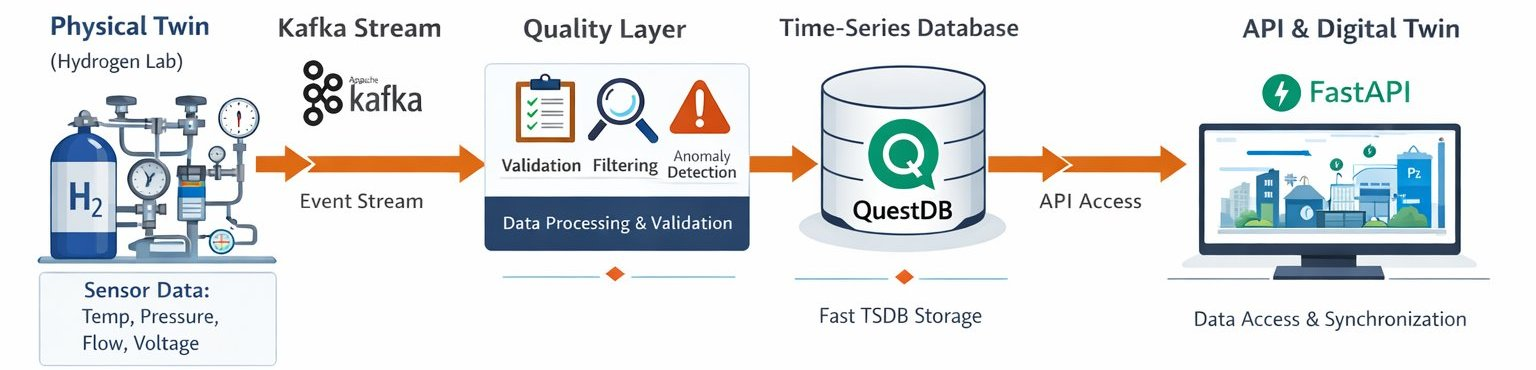
\includegraphics[width=0.95\textwidth]{images/github_internship_image_cropped.jpg}
  \caption{High-level architecture of the Physical-to-Digital Twin pipeline.
           Sensor telemetry flows left to right: simulator $\to$ Kafka $\to$
           ingestion service $\to$ QuestDB $\to$ API and monitoring.}
  \label{fig:pipeline-overview}
\end{figure}

All services are containerised and orchestrated with Docker Compose.
The implementation language is Python~3.11 throughout, with
FastAPI~\cite{fastapi} for the API layer,
confluent-kafka~\cite{confluentkafka} for Kafka connectivity,
PyJWT and bcrypt for authentication, and
structlog~\cite{structlog} for structured logging.

% ============================================================
\section{Physics Simulation Layer}
\label{sec:simulator}
% ============================================================

\subsection{Design rationale}
\label{subsec:sim-rationale}

The physical twin is replaced by a software simulator that reproduces the
dynamic behaviour of the hydrogen production facility described in
Pietra~et~al.~\cite{pietra2021}.
That work characterised a 21.2\,kW alkaline electrolyser (AEL) paired with
an air-driven reciprocating booster compressor filling a 200\,bar\,g
storage vessel, and published time-series data at 1\,Hz for two operating
points: 4.6\,bar\,g back-pressure (2.52\,Nm$^3$/h H$_2$ flow,
93\,kWh/kg specific energy consumption) and 4.2\,bar\,g
(5.53\,Nm$^3$/h, 77\,kWh/kg).

A simulator rather than replay of the recorded data was chosen for three
reasons: (i)~it produces an unbounded stream at any desired rate;
(ii)~it allows deliberate injection of data quality faults; and
(iii)~its parameters can be changed at runtime without modifying any stored
dataset.

\subsection{Sub-model structure}
\label{subsec:sim-structure}

The simulator is implemented in \texttt{simulator/hydrogen\_plant.py} as
four coupled sub-models coordinated by the top-level
\texttt{HydrogenPlantSimulator} class.
Table~\ref{tab:submodels} summarises each sub-model's physical scope and
the paper references used for calibration.

\begin{table}[H]
  \centering
  \caption{Physics simulator sub-models and their calibration sources.}
  \label{tab:submodels}
  \begin{tabularx}{\textwidth}{lXl}
    \toprule
    \textbf{Sub-model} & \textbf{Key behaviour} & \textbf{Reference} \\
    \midrule
    \texttt{ElectrolyserModel}
      & 5-min warm-up ramp; purge dips every 180\,s (8\,s, flow\,$\to$\,15\%
        of nominal); power $\approx$\,21.2\,kW; slow temperature random walk.
      & Figs.~4--5, Table~9 \\[4pt]
    \texttt{CompressorModel}
      & Storage pressure 10\,$\to$\,200\,bar\,g in $\approx$\,5\,h;
        drive-air flow steps 20\,$\to$\,55\,Nm$^3$/h with storage pressure;
        45\,s air-compressor load/unload cycle.
      & Figs.~6--10, Tables~11--12 \\[4pt]
    \texttt{HydrogenBuffer}
      & 50\,L ideal-gas low-pressure buffer between AEL and booster;
        pressure updated from mass balance each tick via
        $p = nRT/(V \cdot 10^5)$.
      & Section~2.1 \\[4pt]
    \texttt{TemperatureModel}
      & Slow independent random walk on nine TT channels within
        physically calibrated bounds; Joule-Thomson cooling reproduced
        on H$_2$ line sensors.
      & Section~2.3.1 \\
    \bottomrule
  \end{tabularx}
\end{table}

\subsection{Streaming interface}
\label{subsec:sim-interface}

The \texttt{HydrogenPlantSimulator.step()} method advances all sub-models
by one time-step $\Delta t$ (default 1\,s) and returns a Python dictionary
whose keys match the pipeline table schema directly (e.g.\
\texttt{H2\_005PT}, \texttt{H2\_001FT}, \texttt{H2\_001TT}).
This allows the producer entry point to remain agnostic of the simulation
internals:

\begin{lstlisting}[language=Python, caption={Producer main loop (cmd/producer.py).},
                   label={lst:producer-loop}]
sim = HydrogenPlantSimulator()
while True:
    state = sim.step()          # one sensor tick
    state["auth"] = {"token": token, "device_id": device_id}
    kafka_client.publish(state) # serialise to JSON and send
    time.sleep(0.5)             # 2 Hz publish rate
\end{lstlisting}

A thin compatibility shim in \texttt{simulator/physics\_model.py} preserves
the original \texttt{initial\_state()} / \texttt{generate\_physical\_state()}
function signatures for backward compatibility.

% ============================================================
\section{Data Streaming Layer}
\label{sec:streaming}
% ============================================================

\subsection{Kafka topology}
\label{subsec:kafka}

Apache Kafka~\cite{kafka} provides the decoupling layer between the
simulator and the ingestion service.
Two topics are used:

\begin{itemize}
  \item \textbf{\texttt{raw\_h2\_data}} — the primary ingest topic.
        Every message published by the producer lands here.
  \item \textbf{\texttt{validated\_h2\_data}} — the table name used as a
        logical label for validated records persisted by the consumer.
        (Not a separate Kafka topic; the consumer writes directly to
        QuestDB after validation.)
\end{itemize}

The Confluent Platform 7.4 Kafka and Zookeeper images are used.
The broker advertises two listeners: \texttt{broker:9092} for
intra-container traffic and \texttt{localhost:29092} for host-side access.

\subsection{Message format}
\label{subsec:message-format}

Each Kafka message is a JSON object containing the 13 sensor readings,
an ISO-8601 UTC timestamp, and a nested authentication block carrying the
device JWT:

\begin{lstlisting}[language=json, caption={Example Kafka message (abridged).},
                   label={lst:kafka-message}]
{
  "timestamp":  "2026-04-25T09:48:01.123456Z",
  "H2_001PT":  -4.002,   // upstream EL, sensor range artefact
  "H2_002PT":   4.491,   // low-pressure buffer (~4.5 bar g)
  "H2_005PT":  13.660,   // storage vessel (rising 10->200 bar g)
  "H2_001FT":   2.527,   // H2 flow from electrolyser [Nm3/h]
  "H2_001TT":  26.977,   // H2 line temperature [C]
  "FC_STATE":  100.0,    // standby-ready
  "auth": { "token": "<JWT>", "device_id": "simulation_device_01" }
}
\end{lstlisting}

% ============================================================
\section{Ingestion and Data Quality Layer}
\label{sec:quality}
% ============================================================

\subsection{Pipeline stages}
\label{subsec:ingestion-pipeline}

The \texttt{IngestionService} (\texttt{services/ingestion\_service.py})
consumes Kafka messages in a tight polling loop and passes each record
through five sequential stages, shown in Figure~\ref{fig:ingestion-flow}.

\begin{enumerate}
  \item \textbf{JWT authentication} — the device token embedded in
        \texttt{data["auth"]["token"]} is verified against the server-side
        secret; records with missing, expired, or insufficient-permission
        tokens are routed to the dead-letter table.
  \item \textbf{Raw persistence} — the authenticated record is inserted into
        \texttt{raw\_h2\_data} immediately, with non-finite float values
        (\texttt{NaN}, \texttt{Inf}) stored as SQL \texttt{NULL} rather than
        rejected.
  \item \textbf{Quality dimension scoring} — all seven dimensions
        (Section~\ref{subsec:quality-dims}) are computed and persisted to
        \texttt{raw\_h2\_data\_quality}.
  \item \textbf{Imputation} — NaN/Inf fields are replaced by the last
        known good value for that field (forward-fill).
  \item \textbf{Validation and routing} — the imputed record is validated;
        passing records go to \texttt{validated\_h2\_data}, failing records
        to the dead-letter table.
\end{enumerate}

\begin{figure}[H]
  \centering
  \begin{verbatim}
  Kafka message
      |
      +-- JWT auth check -----[fail]--> raw_h2_data_dead_letter
      |
      +-- INSERT raw record  ----------> raw_h2_data
      |    (NaN/Inf stored as NULL)
      |
      +-- evaluate_dimensions() -------> raw_h2_data_quality
      |
      +-- clean_record()  [impute NaN]
      |
      +-- validate_record() --[fail]--> raw_h2_data_dead_letter
      |
      +-- INSERT clean record ---------> validated_h2_data
  \end{verbatim}
  \caption{Message routing inside \texttt{IngestionService}.}
  \label{fig:ingestion-flow}
\end{figure}

\subsection{Quality dimensions}
\label{subsec:quality-dims}

The quality assessment framework is implemented in \texttt{domain/quality.py}
following the multi-dimensional model proposed by Peixoto~et~al.~\cite{peixoto2025}.
Seven scalar dimensions are computed per message and stored in
\texttt{raw\_h2\_data\_quality} for retrospective analysis and live
Grafana visualisation.

\paragraph{Completeness ($C$).}
The fraction of non-null fields in the raw record:
\begin{equation}
  C = \frac{|\{f \in \mathcal{F} : v_f \neq \texttt{NULL}\}|}{|\mathcal{F}|}
  \label{eq:completeness}
\end{equation}
where $\mathcal{F}$ is the full set of expected fields.
This is a \emph{per-message} dimension: it requires no historical context.

\paragraph{Timeliness ($T$).}
A linear decay from 1 to 0 over a volatility window $\tau = 120$\,s:
\begin{equation}
  T = \max\!\left(0,\; 1 - \frac{t_{\text{now}} - t_{\text{msg}}}{\tau}\right)
  \label{eq:timeliness}
\end{equation}
A record that is more than two minutes old when it reaches the consumer
scores 0. Under normal operating conditions the consumer lag is under 1\,s,
so $T \approx 1$.

\paragraph{Accuracy ($A$).}
Per-field outlier detection using the Hampel identifier~\cite{hampel1974}
over a rolling window of $W = 60$ readings.
For each field $f$, the fraction of outliers within the window is computed
from the median absolute deviation (MAD):
\begin{equation}
  \hat{\sigma}_f = 1.4826 \cdot \text{MAD}(x_{f,1},\ldots,x_{f,W}),
  \qquad
  \text{outlier if } |x_{f,t} - \tilde{x}_f| > k\,\hat{\sigma}_f
  \label{eq:hampel}
\end{equation}
with $k = 3$. The accuracy score is the mean of $(1 - r_f)$ across all
sensor fields, where $r_f$ is the outlier fraction for field $f$.
This is a \emph{per-window} dimension: it stabilises only after 60 messages.

\paragraph{Temporal completeness ($T_c$).}
\begin{equation}
  T_c = \min\!\left(1,\; \frac{n_{\text{processed}}}{W}\right)
  \label{eq:temporal-completeness}
\end{equation}
This ramps from 0 to 1 as the observation window fills after a consumer
restart, signalling when per-window dimensions become reliable.

\paragraph{Weighted quality score (WQS).}
A weighted combination of accuracy and completeness:
\begin{equation}
  \text{WQS}_t = w_A \cdot A_t + w_C \cdot C_t, \qquad w_A = 0.7,\; w_C = 0.3
  \label{eq:wqs}
\end{equation}
The weights reflect the greater importance of numerical plausibility
over field presence for a sensor network of known topology.

\paragraph{Longitudinal WQS (LWQS).}
An exponentially weighted mean of the WQS history, smoothing transient
noise:
\begin{equation}
  \text{LWQS}_t = \sum_{k=0}^{n-1} \alpha_k \cdot \text{WQS}_{t-k},
  \qquad
  \alpha_k = \frac{e^{-k/\beta}}{\sum_{j=0}^{n-1} e^{-j/\beta}},
  \quad \beta = 5
  \label{eq:lwqs}
\end{equation}

\paragraph{Quality score drift (QSD).}
\begin{equation}
  \text{QSD}_t = \text{WQS}_t - \text{LWQS}_t
  \label{eq:qsd}
\end{equation}
A sustained negative QSD signals that recent quality is below the
established trend — an early warning of sensor degradation or network
problems.

\subsection{Quality storage schema}
\label{subsec:quality-schema}

A dedicated table \texttt{raw\_h2\_data\_quality} is created automatically
by \texttt{IngestionService.setup()} with the following DDL:

\begin{lstlisting}[language=SQL, caption={Quality metrics table DDL (generated by
                   QuestDBClient.create\_table).}, label={lst:quality-ddl}]
CREATE TABLE raw_h2_data_quality (
    timestamp              TIMESTAMP,
    device_id              STRING,
    accuracy               FLOAT,
    completeness           FLOAT,
    temporal_completeness  FLOAT,
    timeliness             FLOAT,
    wqs                    FLOAT,
    lwqs                   FLOAT,
    qsd                    FLOAT
) TIMESTAMP(timestamp) PARTITION BY DAY;
\end{lstlisting}

One row is inserted per consumed Kafka message, giving a 1\,Hz time series
of all seven quality scores that can be queried via the QuestDB PostgreSQL
wire protocol and visualised directly in Grafana.

% ============================================================
\section{Storage Layer}
\label{sec:storage}
% ============================================================

QuestDB~\cite{questdb} is used as the time-series store.
It exposes two interfaces exploited by this project:
an HTTP REST endpoint (\texttt{/exec}) for DDL and SQL queries, and a
PostgreSQL wire protocol on port 8812, used by the Grafana datasource.

All QuestDB interaction is encapsulated in \texttt{infrastructure/questdb/client.py}.
The client deliberately avoids the InfluxDB line-protocol ingress path
(\texttt{/write}) in favour of plain \texttt{INSERT INTO} SQL, which allows
the same \texttt{QuestDBClient} to serve both inserts and schema management
without additional dependencies.

\subsection{Table layout}
\label{subsec:tables}

Three tables are maintained at runtime (Table~\ref{tab:tables}).

\begin{table}[H]
  \centering
  \caption{QuestDB tables and their purpose.}
  \label{tab:tables}
  \begin{tabularx}{\textwidth}{llX}
    \toprule
    \textbf{Table} & \textbf{Rows / msg} & \textbf{Content} \\
    \midrule
    \texttt{raw\_h2\_data}
      & 1
      & Raw record as received; NaN and Inf stored as NULL. \\
    \texttt{validated\_h2\_data}
      & 0 or 1
      & Imputed, validated record; only inserted when all checks pass. \\
    \texttt{raw\_h2\_data\_quality}
      & 1
      & Seven quality dimension scores for the raw record. \\
    \texttt{raw\_h2\_data\_dead\_letter}
      & 0 or 1
      & Sanitised payload of rejected records with failure category and reason. \\
    \bottomrule
  \end{tabularx}
\end{table}

\subsection{NaN and Inf handling}
\label{subsec:nan-handling}

The alkaline electrolyser simulator intentionally injects non-finite values
to model sensor faults (1\% probability of \texttt{NaN} and 1\% probability
of \texttt{Inf} per field per message, configurable via
\texttt{introduce\_issues=True}).
QuestDB's SQL parser rejects bare \texttt{nan} and \texttt{inf} literals
with HTTP~400.
The client guards against this in \texttt{insert\_row}:

\begin{lstlisting}[language=Python,
    caption={NaN/Inf guard in QuestDBClient.insert\_row.},
    label={lst:nan-guard}]
if isinstance(val, (int, float)):
    if not math.isfinite(float(val)):
        continue          # omit column -> stored as NULL
    cols.append(col)
    vals.append(str(val))
\end{lstlisting}

Omitting the column from the INSERT causes QuestDB to store NULL for that
field in \texttt{raw\_h2\_data}.
The imputation step (Section~\ref{subsec:ingestion-pipeline}) then
substitutes the last valid reading before attempting to write to
\texttt{validated\_h2\_data}.

% ============================================================
\section{Authentication and Access Control}
\label{sec:auth}
% ============================================================

Three identity types are supported, all using JWT (JSON Web Tokens)
signed with HS256~\cite{rfc7519}:

\begin{itemize}
  \item \textbf{Device} — sensors authenticate via \texttt{POST /device/login}
        with a pre-shared \texttt{device\_id} and \texttt{device\_secret}
        (bcrypt-hashed at rest).
        The issued token carries
        \texttt{permissions: ["ingest\_data"]} and a 24-hour expiry.
        The producer refreshes the token automatically when fewer than
        300\,s remain.
  \item \textbf{Researcher} — human users authenticate via
        \texttt{POST /researcher/login}.
        The token carries \texttt{roles} and \texttt{data\_access} scopes
        that govern which data types the sync endpoints will return.
  \item \textbf{Admin} — a researcher token with \texttt{"admin"} in
        \texttt{roles}, enforced by the \texttt{get\_admin\_user}
        FastAPI dependency.
\end{itemize}

Credential storage uses two JSON files managed by the
\texttt{JsonFileRepository} implementation of the abstract
\texttt{CredentialRepository} interface
(\texttt{infrastructure/registry/repository.py}), supporting future
migration to a database-backed store without changing service code.

Authentication logic is entirely contained in \texttt{domain/auth.py}
as pure functions that accept the secret as a parameter, making them
trivially unit-testable without any HTTP or database fixtures.

% ============================================================
\section{API Layer}
\label{sec:api}
% ============================================================

The FastAPI application (\texttt{api/main.py}) exposes three router groups,
summarised in Table~\ref{tab:api}.

\begin{table}[H]
  \centering
  \caption{FastAPI router summary.}
  \label{tab:api}
  \begin{tabularx}{\textwidth}{llX}
    \toprule
    \textbf{Endpoint} & \textbf{Method} & \textbf{Description} \\
    \midrule
    \texttt{/device/login}      & POST & Issue device JWT. \\
    \texttt{/researcher/login}  & POST & Issue researcher JWT. \\
    \texttt{/verify}            & POST & Validate any token. \\
    \texttt{/health}            & GET  & Auth service health check. \\
    \midrule
    \texttt{/sync/trigger}      & POST & Sync one paginated batch (researcher). \\
    \texttt{/sync/status}       & GET  & Sync state and available record count. \\
    \texttt{/sync/complete}     & POST & Sync all remaining records. \\
    \midrule
    \texttt{/status}            & GET  & Auto-sync worker state (admin). \\
    \texttt{/trigger}           & POST & Trigger manual sync batch (admin). \\
    \texttt{/remote-sync/test-ssh} & POST & Verify SSH connectivity. \\
    \texttt{/summary}           & GET  & Synced output file listing. \\
    \texttt{/metrics}           & GET  & Prometheus metrics (ASGI mount). \\
    \bottomrule
  \end{tabularx}
\end{table}

A background asyncio task (\texttt{workers/auto\_sync\_worker.py}) is
launched in the FastAPI lifespan hook.
It polls QuestDB every \texttt{SYNC\_INTERVAL} seconds and writes a local
JSON/CSV batch when at least \texttt{BATCH\_SIZE} new records are available.
If \texttt{REMOTE\_SYNC\_ENABLED=true}, the batch is also transferred over
SSH/SFTP to the ORFEO-Hydor research platform using paramiko.

% ============================================================
\section{Monitoring}
\label{sec:monitoring}
% ============================================================

\subsection{Prometheus metrics}
\label{subsec:prometheus}

Two processes expose Prometheus metrics:
\begin{itemize}
  \item The \textbf{Kafka consumer} starts a Prometheus HTTP server on
        port~8001 (\texttt{prometheus\_client.start\_http\_server}).
  \item The \textbf{FastAPI app} mounts the metrics ASGI app at
        \texttt{/metrics}.
\end{itemize}

Five metrics are defined in \texttt{infrastructure/metrics.py}
(Table~\ref{tab:metrics}).

\begin{table}[H]
  \centering
  \caption{Prometheus metrics exposed by the pipeline.}
  \label{tab:metrics}
  \begin{tabularx}{\textwidth}{llX}
    \toprule
    \textbf{Metric name} & \textbf{Type} & \textbf{Description} \\
    \midrule
    \texttt{h2\_ingestion\_messages\_total}
      & Counter
      & Messages received, labelled by \texttt{result}:
        \texttt{received} | \texttt{valid} | \texttt{invalid} |
        \texttt{auth\_failed}. \\
    \texttt{h2\_ingestion\_quality\_yield\_ratio}
      & Gauge
      & Rolling ratio of valid to total received messages. \\
    \texttt{h2\_sync\_batches\_total}
      & Counter
      & Auto-sync batch outcomes, labelled by \texttt{status}. \\
    \texttt{h2\_sync\_records\_synced\_total}
      & Counter
      & Cumulative records successfully synced. \\
    \texttt{h2\_sync\_lag\_seconds}
      & Gauge
      & Seconds since the last successful sync batch. \\
    \bottomrule
  \end{tabularx}
\end{table}

\subsection{Grafana dashboards}
\label{subsec:grafana}

Three dashboards are provisioned automatically from the
\texttt{config/grafana/dashboards/} directory:

\begin{itemize}
  \item \textbf{H2 Pipeline --- Live Telemetry} (\texttt{h2-pipeline}):
        ingestion rate (msg/s), quality yield gauge (green $\geq 95\%$),
        sync lag, and cumulative counters, all from Prometheus.
  \item \textbf{H2 Sensor Data} (\texttt{h2-sensors}):
        per-sensor time series with sensor and table dropdowns.
        Queries run against QuestDB via the PostgreSQL datasource on
        port~8812.
        Users select \texttt{raw\_h2\_data} to inspect raw quality or
        \texttt{validated\_h2\_data} for continuous, imputation-corrected
        signals.
  \item \textbf{H2 Data Quality Dimensions} (\texttt{h2-quality}):
        all seven quality dimension scores over time.
        WQS and LWQS are overlaid on one panel to make the smoothing effect
        visible; QSD is plotted separately with threshold colouring to
        highlight quality degradation events.
\end{itemize}

The QuestDB datasource uses the built-in PostgreSQL plugin
(\texttt{type: postgres}) with \texttt{sslmode: disable} and
\texttt{timescaledb: false}.
Panel queries use \texttt{\$\_\_timeFrom()} and \texttt{\$\_\_timeTo()}
macros rather than \texttt{\$\_\_timeFilter()}, which generates a
\texttt{::timestamptz} cast that QuestDB's PostgreSQL wire implementation
does not support.

% ============================================================
\section{Deployment}
\label{sec:deployment}
% ============================================================

The complete stack is defined in a single \texttt{docker-compose.yml}
(Table~\ref{tab:services}).
All application images are built locally from Dockerfiles in the
\texttt{docker/} directory.
Environment variables are loaded from a \texttt{.env} file; the
\texttt{JWT\_SECRET} and \texttt{DEVICE\_SECRET} variables are required
and have no defaults.

\begin{table}[H]
  \centering
  \caption{Docker Compose services and their exposed ports.}
  \label{tab:services}
  \begin{tabularx}{\textwidth}{llX}
    \toprule
    \textbf{Service} & \textbf{Port(s)} & \textbf{Role} \\
    \midrule
    \texttt{zookeeper}      & 2181       & Kafka metadata coordination. \\
    \texttt{broker}         & 9092, 29092 & Kafka message broker. \\
    \texttt{questdb}        & 9000, 8812 & Time-series database (HTTP + PG). \\
    \texttt{kafka\_producer}& —          & Simulator + Kafka publisher. \\
    \texttt{kafka\_consumer}& 8001       & Ingestion service + Prometheus. \\
    \texttt{fastapi\_app}   & 8080       & REST API + Prometheus \texttt{/metrics}. \\
    \texttt{prometheus}     & 9090       & Metrics scraping and storage. \\
    \texttt{grafana}        & 3000       & Dashboard visualisation. \\
    \bottomrule
  \end{tabularx}
\end{table}

The broker health check (\texttt{kafka-topics --list}) is used as a
Docker Compose dependency gate so that the producer and consumer containers
start only after Kafka is confirmed ready.
The consumer additionally sleeps for 15\,s at startup to allow QuestDB and
the FastAPI app to complete their own initialisation.

% ============================================================
\section{Testing}
\label{sec:testing}
% ============================================================

Unit tests (\texttt{tests/unit/}) cover the three pure-function domains:
authentication (\texttt{test\_auth.py}), data quality
(\texttt{test\_quality.py}), and sync state management
(\texttt{test\_sync\_service.py}).
The 27-test suite requires no external services and runs in under
0.5\,s:

\begin{lstlisting}[language=bash, caption={Running the test suite.},
                   label={lst:tests}]
JWT_SECRET=any-dev-secret python3 -m pytest tests/unit/ -v
\end{lstlisting}

A dead-letter integration test (\texttt{tests/unit/test\_dead\_letter.py})
verifies that records failing authentication and validation are correctly
routed to the dead-letter table without raising exceptions in the main
ingestion loop.

% ============================================================
\section{Summary}
\label{sec:impl-summary}
% ============================================================

This chapter presented the full implementation of the hydrogen plant digital
twin pipeline.
The key design decisions were:

\begin{enumerate}
  \item \textbf{Layered architecture} — each of simulation, streaming,
        quality, storage, and exposition is self-contained and
        independently testable.
  \item \textbf{Physics-grounded simulation} — the simulator reproduces
        quantitative behaviours from a peer-reviewed characterisation of
        the target plant type, giving the generated data scientific credibility.
  \item \textbf{Dual-table storage} — separating raw and validated data
        preserves auditability while giving downstream consumers a clean,
        continuous signal.
  \item \textbf{Persistent quality scoring} — all seven quality dimensions
        are computed per message and stored in a dedicated table, making the
        quality layer observable and retrospectively queryable rather than
        ephemeral.
  \item \textbf{Observable monitoring stack} — Prometheus and Grafana
        provide operational visibility into both pipeline health and data
        quality trends without requiring changes to application code.
\end{enumerate}

% ============================================================
% Bibliography entries (add to main .bib file)
% ============================================================
%
% @article{pietra2021,
%   author  = {Pietra, Andrea and others},
%   title   = {Experimental Characterization of an Alkaline Electrolyser
%              and a Compression System for Hydrogen Production and Storage},
%   journal = {Energies},
%   year    = {2021},
%   volume  = {14},
%   number  = {17},
%   pages   = {5347},
%   doi     = {10.3390/en14175347}
% }
%
% @article{peixoto2025,
%   author  = {Peixoto, ... and others},
%   title   = {Multi-dimensional data quality framework for IoT sensor streams},
%   journal = {???},
%   year    = {2025},
% }
%
% @misc{fastapi,
%   title  = {{FastAPI}},
%   author = {Ramirez, Sebasti\'an},
%   url    = {https://fastapi.tiangolo.com},
%   year   = {2019}
% }
%
% @misc{questdb,
%   title  = {{QuestDB}: Time-Series Database},
%   url    = {https://questdb.io},
%   year   = {2021}
% }
%
% @misc{kafka,
%   title  = {{Apache Kafka}},
%   author = {{Apache Software Foundation}},
%   url    = {https://kafka.apache.org},
%   year   = {2011}
% }
%
% @misc{structlog,
%   title  = {structlog: Structured Logging for Python},
%   url    = {https://www.structlog.org},
%   year   = {2013}
% }
%
% @misc{confluentkafka,
%   title  = {confluent-kafka-python},
%   author = {{Confluent Inc.}},
%   url    = {https://github.com/confluentinc/confluent-kafka-python},
%   year   = {2016}
% }
%
% @misc{rfc7519,
%   author = {Jones, M. and Bradley, J. and Sakimura, N.},
%   title  = {{RFC} 7519: {JSON} Web Token ({JWT})},
%   year   = {2015},
%   url    = {https://www.rfc-editor.org/rfc/rfc7519}
% }
%
% @article{hampel1974,
%   author  = {Hampel, Frank R.},
%   title   = {The Influence Curve and Its Role in Robust Estimation},
%   journal = {Journal of the American Statistical Association},
%   year    = {1974},
%   volume  = {69},
%   number  = {346},
%   pages   = {383--393},
%   doi     = {10.2307/2285666}
% }

% Required packages in preamble:
%   \usepackage{booktabs, tabularx, listings, xcolor, graphicx,
%               hyperref, amsmath, amssymb, float, caption}
% ============================================================

\chapter{Implementation of the Physical-to-Digital Twin Pipeline}
\label{ch:implementation}

\section{Overview}
\label{sec:impl-overview}

This chapter describes the end-to-end implementation of the hydrogen plant
digital twin pipeline.
The system translates continuous sensor output from a simulated alkaline
electrolyser and hydrogen compression plant into a queryable, monitored
time-series database, and exposes the data to authenticated external
consumers through a REST API.

The pipeline follows a layered architecture, illustrated schematically in
Figure~\ref{fig:pipeline-overview}, organised around five concerns:
simulation, streaming, quality assurance, storage, and exposition.
Each layer is independently testable and replaceable.

\begin{figure}[H]
  \centering
  % Replace with actual architecture diagram
  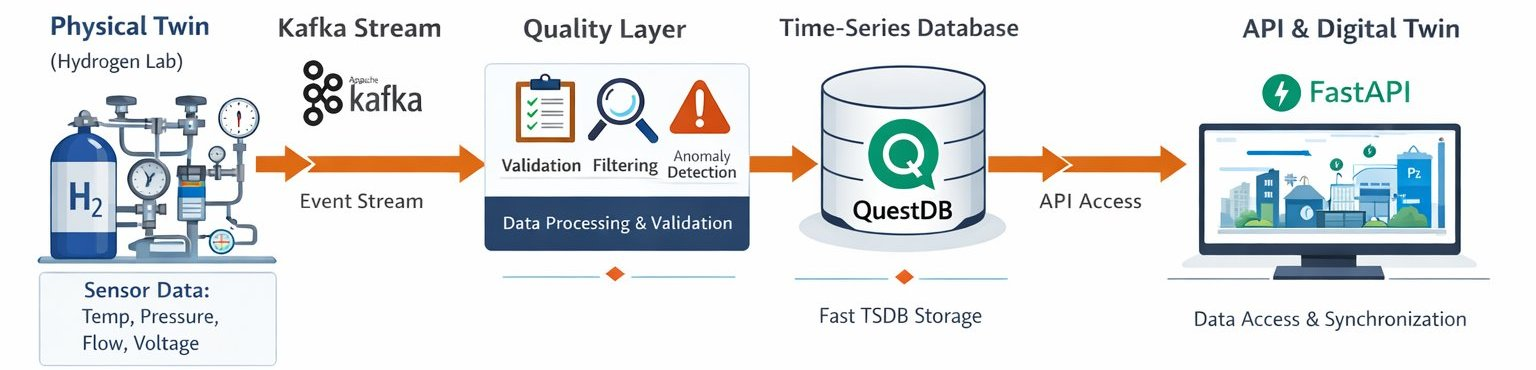
\includegraphics[width=0.95\textwidth]{images/github_internship_image_cropped.jpg}
  \caption{High-level architecture of the Physical-to-Digital Twin pipeline.
           Sensor telemetry flows left to right: simulator $\to$ Kafka $\to$
           ingestion service $\to$ QuestDB $\to$ API and monitoring.}
  \label{fig:pipeline-overview}
\end{figure}

All services are containerised and orchestrated with Docker Compose.
The implementation language is Python~3.11 throughout, with
FastAPI~\cite{fastapi} for the API layer,
confluent-kafka~\cite{confluentkafka} for Kafka connectivity,
PyJWT and bcrypt for authentication, and
structlog~\cite{structlog} for structured logging.

% ============================================================
\section{Physics Simulation Layer}
\label{sec:simulator}
% ============================================================

\subsection{Design rationale}
\label{subsec:sim-rationale}

The physical twin is replaced by a software simulator that reproduces the
dynamic behaviour of the hydrogen production facility described in
Pietra~et~al.~\cite{pietra2021}.
That work characterised a 21.2\,kW alkaline electrolyser (AEL) paired with
an air-driven reciprocating booster compressor filling a 200\,bar\,g
storage vessel, and published time-series data at 1\,Hz for two operating
points: 4.6\,bar\,g back-pressure (2.52\,Nm$^3$/h H$_2$ flow,
93\,kWh/kg specific energy consumption) and 4.2\,bar\,g
(5.53\,Nm$^3$/h, 77\,kWh/kg).

A simulator rather than replay of the recorded data was chosen for three
reasons: (i)~it produces an unbounded stream at any desired rate;
(ii)~it allows deliberate injection of data quality faults; and
(iii)~its parameters can be changed at runtime without modifying any stored
dataset.

\subsection{Sub-model structure}
\label{subsec:sim-structure}

The simulator is implemented in \texttt{simulator/hydrogen\_plant.py} as
four coupled sub-models coordinated by the top-level
\texttt{HydrogenPlantSimulator} class.
Table~\ref{tab:submodels} summarises each sub-model's physical scope and
the paper references used for calibration.

\begin{table}[H]
  \centering
  \caption{Physics simulator sub-models and their calibration sources.}
  \label{tab:submodels}
  \begin{tabularx}{\textwidth}{lXl}
    \toprule
    \textbf{Sub-model} & \textbf{Key behaviour} & \textbf{Reference} \\
    \midrule
    \texttt{ElectrolyserModel}
      & 5-min warm-up ramp; purge dips every 180\,s (8\,s, flow\,$\to$\,15\%
        of nominal); power $\approx$\,21.2\,kW; slow temperature random walk.
      & Figs.~4--5, Table~9 \\[4pt]
    \texttt{CompressorModel}
      & Storage pressure 10\,$\to$\,200\,bar\,g in $\approx$\,5\,h;
        drive-air flow steps 20\,$\to$\,55\,Nm$^3$/h with storage pressure;
        45\,s air-compressor load/unload cycle.
      & Figs.~6--10, Tables~11--12 \\[4pt]
    \texttt{HydrogenBuffer}
      & 50\,L ideal-gas low-pressure buffer between AEL and booster;
        pressure updated from mass balance each tick via
        $p = nRT/(V \cdot 10^5)$.
      & Section~2.1 \\[4pt]
    \texttt{TemperatureModel}
      & Slow independent random walk on nine TT channels within
        physically calibrated bounds; Joule-Thomson cooling reproduced
        on H$_2$ line sensors.
      & Section~2.3.1 \\
    \bottomrule
  \end{tabularx}
\end{table}

\subsection{Streaming interface}
\label{subsec:sim-interface}

The \texttt{HydrogenPlantSimulator.step()} method advances all sub-models
by one time-step $\Delta t$ (default 1\,s) and returns a Python dictionary
whose keys match the pipeline table schema directly (e.g.\
\texttt{H2\_005PT}, \texttt{H2\_001FT}, \texttt{H2\_001TT}).
This allows the producer entry point to remain agnostic of the simulation
internals:

\begin{lstlisting}[language=Python, caption={Producer main loop (cmd/producer.py).},
                   label={lst:producer-loop}]
sim = HydrogenPlantSimulator()
while True:
    state = sim.step()          # one sensor tick
    state["auth"] = {"token": token, "device_id": device_id}
    kafka_client.publish(state) # serialise to JSON and send
    time.sleep(0.5)             # 2 Hz publish rate
\end{lstlisting}

A thin compatibility shim in \texttt{simulator/physics\_model.py} preserves
the original \texttt{initial\_state()} / \texttt{generate\_physical\_state()}
function signatures for backward compatibility.

% ============================================================
\section{Data Streaming Layer}
\label{sec:streaming}
% ============================================================

\subsection{Kafka topology}
\label{subsec:kafka}

Apache Kafka~\cite{kafka} provides the decoupling layer between the
simulator and the ingestion service.
Two topics are used:

\begin{itemize}
  \item \textbf{\texttt{raw\_h2\_data}} — the primary ingest topic.
        Every message published by the producer lands here.
  \item \textbf{\texttt{validated\_h2\_data}} — the table name used as a
        logical label for validated records persisted by the consumer.
        (Not a separate Kafka topic; the consumer writes directly to
        QuestDB after validation.)
\end{itemize}

The Confluent Platform 7.4 Kafka and Zookeeper images are used.
The broker advertises two listeners: \texttt{broker:9092} for
intra-container traffic and \texttt{localhost:29092} for host-side access.

\subsection{Message format}
\label{subsec:message-format}

Each Kafka message is a JSON object containing the 13 sensor readings,
an ISO-8601 UTC timestamp, and a nested authentication block carrying the
device JWT:

\begin{lstlisting}[language=json, caption={Example Kafka message (abridged).},
                   label={lst:kafka-message}]
{
  "timestamp":  "2026-04-25T09:48:01.123456Z",
  "H2_001PT":  -4.002,   // upstream EL, sensor range artefact
  "H2_002PT":   4.491,   // low-pressure buffer (~4.5 bar g)
  "H2_005PT":  13.660,   // storage vessel (rising 10->200 bar g)
  "H2_001FT":   2.527,   // H2 flow from electrolyser [Nm3/h]
  "H2_001TT":  26.977,   // H2 line temperature [C]
  "FC_STATE":  100.0,    // standby-ready
  "auth": { "token": "<JWT>", "device_id": "simulation_device_01" }
}
\end{lstlisting}

% ============================================================
\section{Ingestion and Data Quality Layer}
\label{sec:quality}
% ============================================================

\subsection{Pipeline stages}
\label{subsec:ingestion-pipeline}

The \texttt{IngestionService} (\texttt{services/ingestion\_service.py})
consumes Kafka messages in a tight polling loop and passes each record
through five sequential stages, shown in Figure~\ref{fig:ingestion-flow}.

\begin{enumerate}
  \item \textbf{JWT authentication} — the device token embedded in
        \texttt{data["auth"]["token"]} is verified against the server-side
        secret; records with missing, expired, or insufficient-permission
        tokens are routed to the dead-letter table.
  \item \textbf{Raw persistence} — the authenticated record is inserted into
        \texttt{raw\_h2\_data} immediately, with non-finite float values
        (\texttt{NaN}, \texttt{Inf}) stored as SQL \texttt{NULL} rather than
        rejected.
  \item \textbf{Quality dimension scoring} — all seven dimensions
        (Section~\ref{subsec:quality-dims}) are computed and persisted to
        \texttt{raw\_h2\_data\_quality}.
  \item \textbf{Imputation} — NaN/Inf fields are replaced by the last
        known good value for that field (forward-fill).
  \item \textbf{Validation and routing} — the imputed record is validated;
        passing records go to \texttt{validated\_h2\_data}, failing records
        to the dead-letter table.
\end{enumerate}

\begin{figure}[H]
  \centering
  \begin{verbatim}
  Kafka message
      |
      +-- JWT auth check -----[fail]--> raw_h2_data_dead_letter
      |
      +-- INSERT raw record  ----------> raw_h2_data
      |    (NaN/Inf stored as NULL)
      |
      +-- evaluate_dimensions() -------> raw_h2_data_quality
      |
      +-- clean_record()  [impute NaN]
      |
      +-- validate_record() --[fail]--> raw_h2_data_dead_letter
      |
      +-- INSERT clean record ---------> validated_h2_data
  \end{verbatim}
  \caption{Message routing inside \texttt{IngestionService}.}
  \label{fig:ingestion-flow}
\end{figure}

\subsection{Quality dimensions}
\label{subsec:quality-dims}

The quality assessment framework is implemented in \texttt{domain/quality.py}
following the multi-dimensional model proposed by Peixoto~et~al.~\cite{peixoto2025}.
Seven scalar dimensions are computed per message and stored in
\texttt{raw\_h2\_data\_quality} for retrospective analysis and live
Grafana visualisation.

\paragraph{Completeness ($C$).}
The fraction of non-null fields in the raw record:
\begin{equation}
  C = \frac{|\{f \in \mathcal{F} : v_f \neq \texttt{NULL}\}|}{|\mathcal{F}|}
  \label{eq:completeness}
\end{equation}
where $\mathcal{F}$ is the full set of expected fields.
This is a \emph{per-message} dimension: it requires no historical context.

\paragraph{Timeliness ($T$).}
A linear decay from 1 to 0 over a volatility window $\tau = 120$\,s:
\begin{equation}
  T = \max\!\left(0,\; 1 - \frac{t_{\text{now}} - t_{\text{msg}}}{\tau}\right)
  \label{eq:timeliness}
\end{equation}
A record that is more than two minutes old when it reaches the consumer
scores 0. Under normal operating conditions the consumer lag is under 1\,s,
so $T \approx 1$.

\paragraph{Accuracy ($A$).}
Per-field outlier detection using the Hampel identifier~\cite{hampel1974}
over a rolling window of $W = 60$ readings.
For each field $f$, the fraction of outliers within the window is computed
from the median absolute deviation (MAD):
\begin{equation}
  \hat{\sigma}_f = 1.4826 \cdot \text{MAD}(x_{f,1},\ldots,x_{f,W}),
  \qquad
  \text{outlier if } |x_{f,t} - \tilde{x}_f| > k\,\hat{\sigma}_f
  \label{eq:hampel}
\end{equation}
with $k = 3$. The accuracy score is the mean of $(1 - r_f)$ across all
sensor fields, where $r_f$ is the outlier fraction for field $f$.
This is a \emph{per-window} dimension: it stabilises only after 60 messages.

\paragraph{Temporal completeness ($T_c$).}
\begin{equation}
  T_c = \min\!\left(1,\; \frac{n_{\text{processed}}}{W}\right)
  \label{eq:temporal-completeness}
\end{equation}
This ramps from 0 to 1 as the observation window fills after a consumer
restart, signalling when per-window dimensions become reliable.

\paragraph{Weighted quality score (WQS).}
A weighted combination of accuracy and completeness:
\begin{equation}
  \text{WQS}_t = w_A \cdot A_t + w_C \cdot C_t, \qquad w_A = 0.7,\; w_C = 0.3
  \label{eq:wqs}
\end{equation}
The weights reflect the greater importance of numerical plausibility
over field presence for a sensor network of known topology.

\paragraph{Longitudinal WQS (LWQS).}
An exponentially weighted mean of the WQS history, smoothing transient
noise:
\begin{equation}
  \text{LWQS}_t = \sum_{k=0}^{n-1} \alpha_k \cdot \text{WQS}_{t-k},
  \qquad
  \alpha_k = \frac{e^{-k/\beta}}{\sum_{j=0}^{n-1} e^{-j/\beta}},
  \quad \beta = 5
  \label{eq:lwqs}
\end{equation}

\paragraph{Quality score drift (QSD).}
\begin{equation}
  \text{QSD}_t = \text{WQS}_t - \text{LWQS}_t
  \label{eq:qsd}
\end{equation}
A sustained negative QSD signals that recent quality is below the
established trend — an early warning of sensor degradation or network
problems.

\subsection{Quality storage schema}
\label{subsec:quality-schema}

A dedicated table \texttt{raw\_h2\_data\_quality} is created automatically
by \texttt{IngestionService.setup()} with the following DDL:

\begin{lstlisting}[language=SQL, caption={Quality metrics table DDL (generated by
                   QuestDBClient.create\_table).}, label={lst:quality-ddl}]
CREATE TABLE raw_h2_data_quality (
    timestamp              TIMESTAMP,
    device_id              STRING,
    accuracy               FLOAT,
    completeness           FLOAT,
    temporal_completeness  FLOAT,
    timeliness             FLOAT,
    wqs                    FLOAT,
    lwqs                   FLOAT,
    qsd                    FLOAT
) TIMESTAMP(timestamp) PARTITION BY DAY;
\end{lstlisting}

One row is inserted per consumed Kafka message, giving a 1\,Hz time series
of all seven quality scores that can be queried via the QuestDB PostgreSQL
wire protocol and visualised directly in Grafana.

% ============================================================
\section{Storage Layer}
\label{sec:storage}
% ============================================================

QuestDB~\cite{questdb} is used as the time-series store.
It exposes two interfaces exploited by this project:
an HTTP REST endpoint (\texttt{/exec}) for DDL and SQL queries, and a
PostgreSQL wire protocol on port 8812, used by the Grafana datasource.

All QuestDB interaction is encapsulated in \texttt{infrastructure/questdb/client.py}.
The client deliberately avoids the InfluxDB line-protocol ingress path
(\texttt{/write}) in favour of plain \texttt{INSERT INTO} SQL, which allows
the same \texttt{QuestDBClient} to serve both inserts and schema management
without additional dependencies.

\subsection{Table layout}
\label{subsec:tables}

Three tables are maintained at runtime (Table~\ref{tab:tables}).

\begin{table}[H]
  \centering
  \caption{QuestDB tables and their purpose.}
  \label{tab:tables}
  \begin{tabularx}{\textwidth}{llX}
    \toprule
    \textbf{Table} & \textbf{Rows / msg} & \textbf{Content} \\
    \midrule
    \texttt{raw\_h2\_data}
      & 1
      & Raw record as received; NaN and Inf stored as NULL. \\
    \texttt{validated\_h2\_data}
      & 0 or 1
      & Imputed, validated record; only inserted when all checks pass. \\
    \texttt{raw\_h2\_data\_quality}
      & 1
      & Seven quality dimension scores for the raw record. \\
    \texttt{raw\_h2\_data\_dead\_letter}
      & 0 or 1
      & Sanitised payload of rejected records with failure category and reason. \\
    \bottomrule
  \end{tabularx}
\end{table}

\subsection{NaN and Inf handling}
\label{subsec:nan-handling}

The alkaline electrolyser simulator intentionally injects non-finite values
to model sensor faults (1\% probability of \texttt{NaN} and 1\% probability
of \texttt{Inf} per field per message, configurable via
\texttt{introduce\_issues=True}).
QuestDB's SQL parser rejects bare \texttt{nan} and \texttt{inf} literals
with HTTP~400.
The client guards against this in \texttt{insert\_row}:

\begin{lstlisting}[language=Python,
    caption={NaN/Inf guard in QuestDBClient.insert\_row.},
    label={lst:nan-guard}]
if isinstance(val, (int, float)):
    if not math.isfinite(float(val)):
        continue          # omit column -> stored as NULL
    cols.append(col)
    vals.append(str(val))
\end{lstlisting}

Omitting the column from the INSERT causes QuestDB to store NULL for that
field in \texttt{raw\_h2\_data}.
The imputation step (Section~\ref{subsec:ingestion-pipeline}) then
substitutes the last valid reading before attempting to write to
\texttt{validated\_h2\_data}.

% ============================================================
\section{Authentication and Access Control}
\label{sec:auth}
% ============================================================

Three identity types are supported, all using JWT (JSON Web Tokens)
signed with HS256~\cite{rfc7519}:

\begin{itemize}
  \item \textbf{Device} — sensors authenticate via \texttt{POST /device/login}
        with a pre-shared \texttt{device\_id} and \texttt{device\_secret}
        (bcrypt-hashed at rest).
        The issued token carries
        \texttt{permissions: ["ingest\_data"]} and a 24-hour expiry.
        The producer refreshes the token automatically when fewer than
        300\,s remain.
  \item \textbf{Researcher} — human users authenticate via
        \texttt{POST /researcher/login}.
        The token carries \texttt{roles} and \texttt{data\_access} scopes
        that govern which data types the sync endpoints will return.
  \item \textbf{Admin} — a researcher token with \texttt{"admin"} in
        \texttt{roles}, enforced by the \texttt{get\_admin\_user}
        FastAPI dependency.
\end{itemize}

Credential storage uses two JSON files managed by the
\texttt{JsonFileRepository} implementation of the abstract
\texttt{CredentialRepository} interface
(\texttt{infrastructure/registry/repository.py}), supporting future
migration to a database-backed store without changing service code.

Authentication logic is entirely contained in \texttt{domain/auth.py}
as pure functions that accept the secret as a parameter, making them
trivially unit-testable without any HTTP or database fixtures.

% ============================================================
\section{API Layer}
\label{sec:api}
% ============================================================

The FastAPI application (\texttt{api/main.py}) exposes three router groups,
summarised in Table~\ref{tab:api}.

\begin{table}[H]
  \centering
  \caption{FastAPI router summary.}
  \label{tab:api}
  \begin{tabularx}{\textwidth}{llX}
    \toprule
    \textbf{Endpoint} & \textbf{Method} & \textbf{Description} \\
    \midrule
    \texttt{/device/login}      & POST & Issue device JWT. \\
    \texttt{/researcher/login}  & POST & Issue researcher JWT. \\
    \texttt{/verify}            & POST & Validate any token. \\
    \texttt{/health}            & GET  & Auth service health check. \\
    \midrule
    \texttt{/sync/trigger}      & POST & Sync one paginated batch (researcher). \\
    \texttt{/sync/status}       & GET  & Sync state and available record count. \\
    \texttt{/sync/complete}     & POST & Sync all remaining records. \\
    \midrule
    \texttt{/status}            & GET  & Auto-sync worker state (admin). \\
    \texttt{/trigger}           & POST & Trigger manual sync batch (admin). \\
    \texttt{/remote-sync/test-ssh} & POST & Verify SSH connectivity. \\
    \texttt{/summary}           & GET  & Synced output file listing. \\
    \texttt{/metrics}           & GET  & Prometheus metrics (ASGI mount). \\
    \bottomrule
  \end{tabularx}
\end{table}

A background asyncio task (\texttt{workers/auto\_sync\_worker.py}) is
launched in the FastAPI lifespan hook.
It polls QuestDB every \texttt{SYNC\_INTERVAL} seconds and writes a local
JSON/CSV batch when at least \texttt{BATCH\_SIZE} new records are available.
If \texttt{REMOTE\_SYNC\_ENABLED=true}, the batch is also transferred over
SSH/SFTP to the ORFEO-Hydor research platform using paramiko.

% ============================================================
\section{Monitoring}
\label{sec:monitoring}
% ============================================================

\subsection{Prometheus metrics}
\label{subsec:prometheus}

Two processes expose Prometheus metrics:
\begin{itemize}
  \item The \textbf{Kafka consumer} starts a Prometheus HTTP server on
        port~8001 (\texttt{prometheus\_client.start\_http\_server}).
  \item The \textbf{FastAPI app} mounts the metrics ASGI app at
        \texttt{/metrics}.
\end{itemize}

Five metrics are defined in \texttt{infrastructure/metrics.py}
(Table~\ref{tab:metrics}).

\begin{table}[H]
  \centering
  \caption{Prometheus metrics exposed by the pipeline.}
  \label{tab:metrics}
  \begin{tabularx}{\textwidth}{llX}
    \toprule
    \textbf{Metric name} & \textbf{Type} & \textbf{Description} \\
    \midrule
    \texttt{h2\_ingestion\_messages\_total}
      & Counter
      & Messages received, labelled by \texttt{result}:
        \texttt{received} | \texttt{valid} | \texttt{invalid} |
        \texttt{auth\_failed}. \\
    \texttt{h2\_ingestion\_quality\_yield\_ratio}
      & Gauge
      & Rolling ratio of valid to total received messages. \\
    \texttt{h2\_sync\_batches\_total}
      & Counter
      & Auto-sync batch outcomes, labelled by \texttt{status}. \\
    \texttt{h2\_sync\_records\_synced\_total}
      & Counter
      & Cumulative records successfully synced. \\
    \texttt{h2\_sync\_lag\_seconds}
      & Gauge
      & Seconds since the last successful sync batch. \\
    \bottomrule
  \end{tabularx}
\end{table}

\subsection{Grafana dashboards}
\label{subsec:grafana}

Three dashboards are provisioned automatically from the
\texttt{config/grafana/dashboards/} directory:

\begin{itemize}
  \item \textbf{H2 Pipeline --- Live Telemetry} (\texttt{h2-pipeline}):
        ingestion rate (msg/s), quality yield gauge (green $\geq 95\%$),
        sync lag, and cumulative counters, all from Prometheus.
  \item \textbf{H2 Sensor Data} (\texttt{h2-sensors}):
        per-sensor time series with sensor and table dropdowns.
        Queries run against QuestDB via the PostgreSQL datasource on
        port~8812.
        Users select \texttt{raw\_h2\_data} to inspect raw quality or
        \texttt{validated\_h2\_data} for continuous, imputation-corrected
        signals.
  \item \textbf{H2 Data Quality Dimensions} (\texttt{h2-quality}):
        all seven quality dimension scores over time.
        WQS and LWQS are overlaid on one panel to make the smoothing effect
        visible; QSD is plotted separately with threshold colouring to
        highlight quality degradation events.
\end{itemize}

The QuestDB datasource uses the built-in PostgreSQL plugin
(\texttt{type: postgres}) with \texttt{sslmode: disable} and
\texttt{timescaledb: false}.
Panel queries use \texttt{\$\_\_timeFrom()} and \texttt{\$\_\_timeTo()}
macros rather than \texttt{\$\_\_timeFilter()}, which generates a
\texttt{::timestamptz} cast that QuestDB's PostgreSQL wire implementation
does not support.

% ============================================================
\section{Deployment}
\label{sec:deployment}
% ============================================================

The complete stack is defined in a single \texttt{docker-compose.yml}
(Table~\ref{tab:services}).
All application images are built locally from Dockerfiles in the
\texttt{docker/} directory.
Environment variables are loaded from a \texttt{.env} file; the
\texttt{JWT\_SECRET} and \texttt{DEVICE\_SECRET} variables are required
and have no defaults.

\begin{table}[H]
  \centering
  \caption{Docker Compose services and their exposed ports.}
  \label{tab:services}
  \begin{tabularx}{\textwidth}{llX}
    \toprule
    \textbf{Service} & \textbf{Port(s)} & \textbf{Role} \\
    \midrule
    \texttt{zookeeper}      & 2181       & Kafka metadata coordination. \\
    \texttt{broker}         & 9092, 29092 & Kafka message broker. \\
    \texttt{questdb}        & 9000, 8812 & Time-series database (HTTP + PG). \\
    \texttt{kafka\_producer}& —          & Simulator + Kafka publisher. \\
    \texttt{kafka\_consumer}& 8001       & Ingestion service + Prometheus. \\
    \texttt{fastapi\_app}   & 8080       & REST API + Prometheus \texttt{/metrics}. \\
    \texttt{prometheus}     & 9090       & Metrics scraping and storage. \\
    \texttt{grafana}        & 3000       & Dashboard visualisation. \\
    \bottomrule
  \end{tabularx}
\end{table}

The broker health check (\texttt{kafka-topics --list}) is used as a
Docker Compose dependency gate so that the producer and consumer containers
start only after Kafka is confirmed ready.
The consumer additionally sleeps for 15\,s at startup to allow QuestDB and
the FastAPI app to complete their own initialisation.

% ============================================================
\section{Testing}
\label{sec:testing}
% ============================================================

Unit tests (\texttt{tests/unit/}) cover the three pure-function domains:
authentication (\texttt{test\_auth.py}), data quality
(\texttt{test\_quality.py}), and sync state management
(\texttt{test\_sync\_service.py}).
The 27-test suite requires no external services and runs in under
0.5\,s:

\begin{lstlisting}[language=bash, caption={Running the test suite.},
                   label={lst:tests}]
JWT_SECRET=any-dev-secret python3 -m pytest tests/unit/ -v
\end{lstlisting}

A dead-letter integration test (\texttt{tests/unit/test\_dead\_letter.py})
verifies that records failing authentication and validation are correctly
routed to the dead-letter table without raising exceptions in the main
ingestion loop.

% ============================================================
\section{Summary}
\label{sec:impl-summary}
% ============================================================

This chapter presented the full implementation of the hydrogen plant digital
twin pipeline.
The key design decisions were:

\begin{enumerate}
  \item \textbf{Layered architecture} — each of simulation, streaming,
        quality, storage, and exposition is self-contained and
        independently testable.
  \item \textbf{Physics-grounded simulation} — the simulator reproduces
        quantitative behaviours from a peer-reviewed characterisation of
        the target plant type, giving the generated data scientific credibility.
  \item \textbf{Dual-table storage} — separating raw and validated data
        preserves auditability while giving downstream consumers a clean,
        continuous signal.
  \item \textbf{Persistent quality scoring} — all seven quality dimensions
        are computed per message and stored in a dedicated table, making the
        quality layer observable and retrospectively queryable rather than
        ephemeral.
  \item \textbf{Observable monitoring stack} — Prometheus and Grafana
        provide operational visibility into both pipeline health and data
        quality trends without requiring changes to application code.
\end{enumerate}

% ============================================================
% Bibliography entries (add to main .bib file)
% ============================================================
%
% @article{pietra2021,
%   author  = {Pietra, Andrea and others},
%   title   = {Experimental Characterization of an Alkaline Electrolyser
%              and a Compression System for Hydrogen Production and Storage},
%   journal = {Energies},
%   year    = {2021},
%   volume  = {14},
%   number  = {17},
%   pages   = {5347},
%   doi     = {10.3390/en14175347}
% }
%
% @article{peixoto2025,
%   author  = {Peixoto, ... and others},
%   title   = {Multi-dimensional data quality framework for IoT sensor streams},
%   journal = {???},
%   year    = {2025},
% }
%
% @misc{fastapi,
%   title  = {{FastAPI}},
%   author = {Ramirez, Sebasti\'an},
%   url    = {https://fastapi.tiangolo.com},
%   year   = {2019}
% }
%
% @misc{questdb,
%   title  = {{QuestDB}: Time-Series Database},
%   url    = {https://questdb.io},
%   year   = {2021}
% }
%
% @misc{kafka,
%   title  = {{Apache Kafka}},
%   author = {{Apache Software Foundation}},
%   url    = {https://kafka.apache.org},
%   year   = {2011}
% }
%
% @misc{structlog,
%   title  = {structlog: Structured Logging for Python},
%   url    = {https://www.structlog.org},
%   year   = {2013}
% }
%
% @misc{confluentkafka,
%   title  = {confluent-kafka-python},
%   author = {{Confluent Inc.}},
%   url    = {https://github.com/confluentinc/confluent-kafka-python},
%   year   = {2016}
% }
%
% @misc{rfc7519,
%   author = {Jones, M. and Bradley, J. and Sakimura, N.},
%   title  = {{RFC} 7519: {JSON} Web Token ({JWT})},
%   year   = {2015},
%   url    = {https://www.rfc-editor.org/rfc/rfc7519}
% }
%
% @article{hampel1974,
%   author  = {Hampel, Frank R.},
%   title   = {The Influence Curve and Its Role in Robust Estimation},
%   journal = {Journal of the American Statistical Association},
%   year    = {1974},
%   volume  = {69},
%   number  = {346},
%   pages   = {383--393},
%   doi     = {10.2307/2285666}
% }

% Required packages in preamble:
%   \usepackage{booktabs, tabularx, listings, xcolor, graphicx,
%               hyperref, amsmath, amssymb, float, caption}
% ============================================================

\chapter{Implementation of the Physical-to-Digital Twin Pipeline}
\label{ch:implementation}

\section{Overview}
\label{sec:impl-overview}

This chapter describes the end-to-end implementation of the hydrogen plant
digital twin pipeline.
The system translates continuous sensor output from a simulated alkaline
electrolyser and hydrogen compression plant into a queryable, monitored
time-series database, and exposes the data to authenticated external
consumers through a REST API.

The pipeline follows a layered architecture, illustrated schematically in
Figure~\ref{fig:pipeline-overview}, organised around five concerns:
simulation, streaming, quality assurance, storage, and exposition.
Each layer is independently testable and replaceable.

\begin{figure}[H]
  \centering
  % Replace with actual architecture diagram
  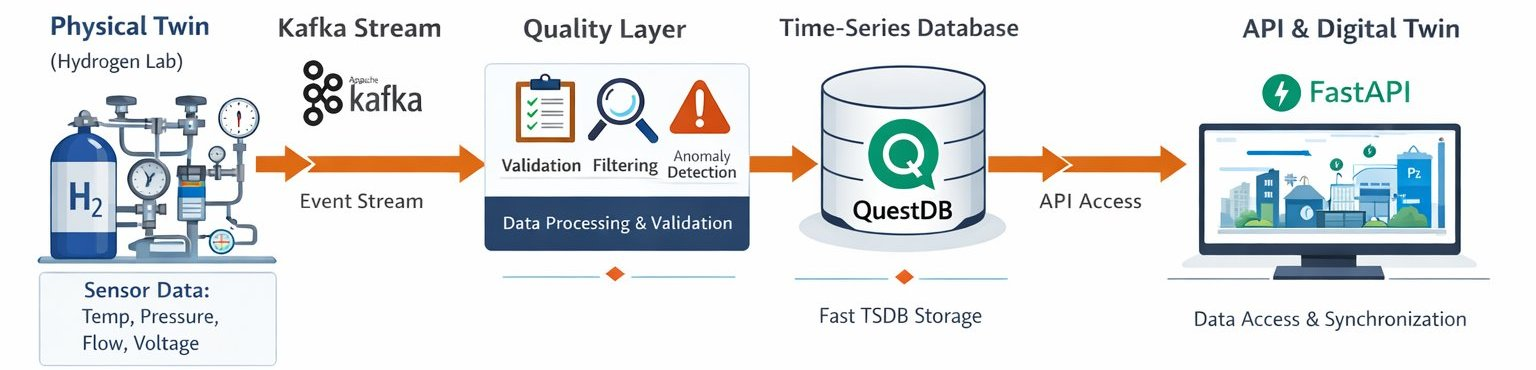
\includegraphics[width=0.95\textwidth]{images/github_internship_image_cropped.jpg}
  \caption{High-level architecture of the Physical-to-Digital Twin pipeline.
           Sensor telemetry flows left to right: simulator $\to$ Kafka $\to$
           ingestion service $\to$ QuestDB $\to$ API and monitoring.}
  \label{fig:pipeline-overview}
\end{figure}

All services are containerised and orchestrated with Docker Compose.
The implementation language is Python~3.11 throughout, with
FastAPI~\cite{fastapi} for the API layer,
confluent-kafka~\cite{confluentkafka} for Kafka connectivity,
PyJWT and bcrypt for authentication, and
structlog~\cite{structlog} for structured logging.

% ============================================================
\section{Physics Simulation Layer}
\label{sec:simulator}
% ============================================================

\subsection{Design rationale}
\label{subsec:sim-rationale}

The physical twin is replaced by a software simulator that reproduces the
dynamic behaviour of the hydrogen production facility described in
Pietra~et~al.~\cite{pietra2021}.
That work characterised a 21.2\,kW alkaline electrolyser (AEL) paired with
an air-driven reciprocating booster compressor filling a 200\,bar\,g
storage vessel, and published time-series data at 1\,Hz for two operating
points: 4.6\,bar\,g back-pressure (2.52\,Nm$^3$/h H$_2$ flow,
93\,kWh/kg specific energy consumption) and 4.2\,bar\,g
(5.53\,Nm$^3$/h, 77\,kWh/kg).

A simulator rather than replay of the recorded data was chosen for three
reasons: (i)~it produces an unbounded stream at any desired rate;
(ii)~it allows deliberate injection of data quality faults; and
(iii)~its parameters can be changed at runtime without modifying any stored
dataset.

\subsection{Sub-model structure}
\label{subsec:sim-structure}

The simulator is implemented in \texttt{simulator/hydrogen\_plant.py} as
four coupled sub-models coordinated by the top-level
\texttt{HydrogenPlantSimulator} class.
Table~\ref{tab:submodels} summarises each sub-model's physical scope and
the paper references used for calibration.

\begin{table}[H]
  \centering
  \caption{Physics simulator sub-models and their calibration sources.}
  \label{tab:submodels}
  \begin{tabularx}{\textwidth}{lXl}
    \toprule
    \textbf{Sub-model} & \textbf{Key behaviour} & \textbf{Reference} \\
    \midrule
    \texttt{ElectrolyserModel}
      & 5-min warm-up ramp; purge dips every 180\,s (8\,s, flow\,$\to$\,15\%
        of nominal); power $\approx$\,21.2\,kW; slow temperature random walk.
      & Figs.~4--5, Table~9 \\[4pt]
    \texttt{CompressorModel}
      & Storage pressure 10\,$\to$\,200\,bar\,g in $\approx$\,5\,h;
        drive-air flow steps 20\,$\to$\,55\,Nm$^3$/h with storage pressure;
        45\,s air-compressor load/unload cycle.
      & Figs.~6--10, Tables~11--12 \\[4pt]
    \texttt{HydrogenBuffer}
      & 50\,L ideal-gas low-pressure buffer between AEL and booster;
        pressure updated from mass balance each tick via
        $p = nRT/(V \cdot 10^5)$.
      & Section~2.1 \\[4pt]
    \texttt{TemperatureModel}
      & Slow independent random walk on nine TT channels within
        physically calibrated bounds; Joule-Thomson cooling reproduced
        on H$_2$ line sensors.
      & Section~2.3.1 \\
    \bottomrule
  \end{tabularx}
\end{table}

\subsection{Streaming interface}
\label{subsec:sim-interface}

The \texttt{HydrogenPlantSimulator.step()} method advances all sub-models
by one time-step $\Delta t$ (default 1\,s) and returns a Python dictionary
whose keys match the pipeline table schema directly (e.g.\
\texttt{H2\_005PT}, \texttt{H2\_001FT}, \texttt{H2\_001TT}).
This allows the producer entry point to remain agnostic of the simulation
internals:

\begin{lstlisting}[language=Python, caption={Producer main loop (cmd/producer.py).},
                   label={lst:producer-loop}]
sim = HydrogenPlantSimulator()
while True:
    state = sim.step()          # one sensor tick
    state["auth"] = {"token": token, "device_id": device_id}
    kafka_client.publish(state) # serialise to JSON and send
    time.sleep(0.5)             # 2 Hz publish rate
\end{lstlisting}

A thin compatibility shim in \texttt{simulator/physics\_model.py} preserves
the original \texttt{initial\_state()} / \texttt{generate\_physical\_state()}
function signatures for backward compatibility.

% ============================================================
\section{Data Streaming Layer}
\label{sec:streaming}
% ============================================================

\subsection{Kafka topology}
\label{subsec:kafka}

Apache Kafka~\cite{kafka} provides the decoupling layer between the
simulator and the ingestion service.
Two topics are used:

\begin{itemize}
  \item \textbf{\texttt{raw\_h2\_data}} — the primary ingest topic.
        Every message published by the producer lands here.
  \item \textbf{\texttt{validated\_h2\_data}} — the table name used as a
        logical label for validated records persisted by the consumer.
        (Not a separate Kafka topic; the consumer writes directly to
        QuestDB after validation.)
\end{itemize}

The Confluent Platform 7.4 Kafka and Zookeeper images are used.
The broker advertises two listeners: \texttt{broker:9092} for
intra-container traffic and \texttt{localhost:29092} for host-side access.

\subsection{Message format}
\label{subsec:message-format}

Each Kafka message is a JSON object containing the 13 sensor readings,
an ISO-8601 UTC timestamp, and a nested authentication block carrying the
device JWT:

\begin{lstlisting}[language=json, caption={Example Kafka message (abridged).},
                   label={lst:kafka-message}]
{
  "timestamp":  "2026-04-25T09:48:01.123456Z",
  "H2_001PT":  -4.002,   // upstream EL, sensor range artefact
  "H2_002PT":   4.491,   // low-pressure buffer (~4.5 bar g)
  "H2_005PT":  13.660,   // storage vessel (rising 10->200 bar g)
  "H2_001FT":   2.527,   // H2 flow from electrolyser [Nm3/h]
  "H2_001TT":  26.977,   // H2 line temperature [C]
  "FC_STATE":  100.0,    // standby-ready
  "auth": { "token": "<JWT>", "device_id": "simulation_device_01" }
}
\end{lstlisting}

% ============================================================
\section{Ingestion and Data Quality Layer}
\label{sec:quality}
% ============================================================

\subsection{Pipeline stages}
\label{subsec:ingestion-pipeline}

The \texttt{IngestionService} (\texttt{services/ingestion\_service.py})
consumes Kafka messages in a tight polling loop and passes each record
through five sequential stages, shown in Figure~\ref{fig:ingestion-flow}.

\begin{enumerate}
  \item \textbf{JWT authentication} — the device token embedded in
        \texttt{data["auth"]["token"]} is verified against the server-side
        secret; records with missing, expired, or insufficient-permission
        tokens are routed to the dead-letter table.
  \item \textbf{Raw persistence} — the authenticated record is inserted into
        \texttt{raw\_h2\_data} immediately, with non-finite float values
        (\texttt{NaN}, \texttt{Inf}) stored as SQL \texttt{NULL} rather than
        rejected.
  \item \textbf{Quality dimension scoring} — all seven dimensions
        (Section~\ref{subsec:quality-dims}) are computed and persisted to
        \texttt{raw\_h2\_data\_quality}.
  \item \textbf{Imputation} — NaN/Inf fields are replaced by the last
        known good value for that field (forward-fill).
  \item \textbf{Validation and routing} — the imputed record is validated;
        passing records go to \texttt{validated\_h2\_data}, failing records
        to the dead-letter table.
\end{enumerate}

\begin{figure}[H]
  \centering
  \begin{verbatim}
  Kafka message
      |
      +-- JWT auth check -----[fail]--> raw_h2_data_dead_letter
      |
      +-- INSERT raw record  ----------> raw_h2_data
      |    (NaN/Inf stored as NULL)
      |
      +-- evaluate_dimensions() -------> raw_h2_data_quality
      |
      +-- clean_record()  [impute NaN]
      |
      +-- validate_record() --[fail]--> raw_h2_data_dead_letter
      |
      +-- INSERT clean record ---------> validated_h2_data
  \end{verbatim}
  \caption{Message routing inside \texttt{IngestionService}.}
  \label{fig:ingestion-flow}
\end{figure}

\subsection{Quality dimensions}
\label{subsec:quality-dims}

The quality assessment framework is implemented in \texttt{domain/quality.py}
following the multi-dimensional model proposed by Peixoto~et~al.~\cite{peixoto2025}.
Seven scalar dimensions are computed per message and stored in
\texttt{raw\_h2\_data\_quality} for retrospective analysis and live
Grafana visualisation.

\paragraph{Completeness ($C$).}
The fraction of non-null fields in the raw record:
\begin{equation}
  C = \frac{|\{f \in \mathcal{F} : v_f \neq \texttt{NULL}\}|}{|\mathcal{F}|}
  \label{eq:completeness}
\end{equation}
where $\mathcal{F}$ is the full set of expected fields.
This is a \emph{per-message} dimension: it requires no historical context.

\paragraph{Timeliness ($T$).}
A linear decay from 1 to 0 over a volatility window $\tau = 120$\,s:
\begin{equation}
  T = \max\!\left(0,\; 1 - \frac{t_{\text{now}} - t_{\text{msg}}}{\tau}\right)
  \label{eq:timeliness}
\end{equation}
A record that is more than two minutes old when it reaches the consumer
scores 0. Under normal operating conditions the consumer lag is under 1\,s,
so $T \approx 1$.

\paragraph{Accuracy ($A$).}
Per-field outlier detection using the Hampel identifier~\cite{hampel1974}
over a rolling window of $W = 60$ readings.
For each field $f$, the fraction of outliers within the window is computed
from the median absolute deviation (MAD):
\begin{equation}
  \hat{\sigma}_f = 1.4826 \cdot \text{MAD}(x_{f,1},\ldots,x_{f,W}),
  \qquad
  \text{outlier if } |x_{f,t} - \tilde{x}_f| > k\,\hat{\sigma}_f
  \label{eq:hampel}
\end{equation}
with $k = 3$. The accuracy score is the mean of $(1 - r_f)$ across all
sensor fields, where $r_f$ is the outlier fraction for field $f$.
This is a \emph{per-window} dimension: it stabilises only after 60 messages.

\paragraph{Temporal completeness ($T_c$).}
\begin{equation}
  T_c = \min\!\left(1,\; \frac{n_{\text{processed}}}{W}\right)
  \label{eq:temporal-completeness}
\end{equation}
This ramps from 0 to 1 as the observation window fills after a consumer
restart, signalling when per-window dimensions become reliable.

\paragraph{Weighted quality score (WQS).}
A weighted combination of accuracy and completeness:
\begin{equation}
  \text{WQS}_t = w_A \cdot A_t + w_C \cdot C_t, \qquad w_A = 0.7,\; w_C = 0.3
  \label{eq:wqs}
\end{equation}
The weights reflect the greater importance of numerical plausibility
over field presence for a sensor network of known topology.

\paragraph{Longitudinal WQS (LWQS).}
An exponentially weighted mean of the WQS history, smoothing transient
noise:
\begin{equation}
  \text{LWQS}_t = \sum_{k=0}^{n-1} \alpha_k \cdot \text{WQS}_{t-k},
  \qquad
  \alpha_k = \frac{e^{-k/\beta}}{\sum_{j=0}^{n-1} e^{-j/\beta}},
  \quad \beta = 5
  \label{eq:lwqs}
\end{equation}

\paragraph{Quality score drift (QSD).}
\begin{equation}
  \text{QSD}_t = \text{WQS}_t - \text{LWQS}_t
  \label{eq:qsd}
\end{equation}
A sustained negative QSD signals that recent quality is below the
established trend — an early warning of sensor degradation or network
problems.

\subsection{Quality storage schema}
\label{subsec:quality-schema}

A dedicated table \texttt{raw\_h2\_data\_quality} is created automatically
by \texttt{IngestionService.setup()} with the following DDL:

\begin{lstlisting}[language=SQL, caption={Quality metrics table DDL (generated by
                   QuestDBClient.create\_table).}, label={lst:quality-ddl}]
CREATE TABLE raw_h2_data_quality (
    timestamp              TIMESTAMP,
    device_id              STRING,
    accuracy               FLOAT,
    completeness           FLOAT,
    temporal_completeness  FLOAT,
    timeliness             FLOAT,
    wqs                    FLOAT,
    lwqs                   FLOAT,
    qsd                    FLOAT
) TIMESTAMP(timestamp) PARTITION BY DAY;
\end{lstlisting}

One row is inserted per consumed Kafka message, giving a 1\,Hz time series
of all seven quality scores that can be queried via the QuestDB PostgreSQL
wire protocol and visualised directly in Grafana.

% ============================================================
\section{Storage Layer}
\label{sec:storage}
% ============================================================

QuestDB~\cite{questdb} is used as the time-series store.
It exposes two interfaces exploited by this project:
an HTTP REST endpoint (\texttt{/exec}) for DDL and SQL queries, and a
PostgreSQL wire protocol on port 8812, used by the Grafana datasource.

All QuestDB interaction is encapsulated in \texttt{infrastructure/questdb/client.py}.
The client deliberately avoids the InfluxDB line-protocol ingress path
(\texttt{/write}) in favour of plain \texttt{INSERT INTO} SQL, which allows
the same \texttt{QuestDBClient} to serve both inserts and schema management
without additional dependencies.

\subsection{Table layout}
\label{subsec:tables}

Three tables are maintained at runtime (Table~\ref{tab:tables}).

\begin{table}[H]
  \centering
  \caption{QuestDB tables and their purpose.}
  \label{tab:tables}
  \begin{tabularx}{\textwidth}{llX}
    \toprule
    \textbf{Table} & \textbf{Rows / msg} & \textbf{Content} \\
    \midrule
    \texttt{raw\_h2\_data}
      & 1
      & Raw record as received; NaN and Inf stored as NULL. \\
    \texttt{validated\_h2\_data}
      & 0 or 1
      & Imputed, validated record; only inserted when all checks pass. \\
    \texttt{raw\_h2\_data\_quality}
      & 1
      & Seven quality dimension scores for the raw record. \\
    \texttt{raw\_h2\_data\_dead\_letter}
      & 0 or 1
      & Sanitised payload of rejected records with failure category and reason. \\
    \bottomrule
  \end{tabularx}
\end{table}

\subsection{NaN and Inf handling}
\label{subsec:nan-handling}

The alkaline electrolyser simulator intentionally injects non-finite values
to model sensor faults (1\% probability of \texttt{NaN} and 1\% probability
of \texttt{Inf} per field per message, configurable via
\texttt{introduce\_issues=True}).
QuestDB's SQL parser rejects bare \texttt{nan} and \texttt{inf} literals
with HTTP~400.
The client guards against this in \texttt{insert\_row}:

\begin{lstlisting}[language=Python,
    caption={NaN/Inf guard in QuestDBClient.insert\_row.},
    label={lst:nan-guard}]
if isinstance(val, (int, float)):
    if not math.isfinite(float(val)):
        continue          # omit column -> stored as NULL
    cols.append(col)
    vals.append(str(val))
\end{lstlisting}

Omitting the column from the INSERT causes QuestDB to store NULL for that
field in \texttt{raw\_h2\_data}.
The imputation step (Section~\ref{subsec:ingestion-pipeline}) then
substitutes the last valid reading before attempting to write to
\texttt{validated\_h2\_data}.

% ============================================================
\section{Authentication and Access Control}
\label{sec:auth}
% ============================================================

Three identity types are supported, all using JWT (JSON Web Tokens)
signed with HS256~\cite{rfc7519}:

\begin{itemize}
  \item \textbf{Device} — sensors authenticate via \texttt{POST /device/login}
        with a pre-shared \texttt{device\_id} and \texttt{device\_secret}
        (bcrypt-hashed at rest).
        The issued token carries
        \texttt{permissions: ["ingest\_data"]} and a 24-hour expiry.
        The producer refreshes the token automatically when fewer than
        300\,s remain.
  \item \textbf{Researcher} — human users authenticate via
        \texttt{POST /researcher/login}.
        The token carries \texttt{roles} and \texttt{data\_access} scopes
        that govern which data types the sync endpoints will return.
  \item \textbf{Admin} — a researcher token with \texttt{"admin"} in
        \texttt{roles}, enforced by the \texttt{get\_admin\_user}
        FastAPI dependency.
\end{itemize}

Credential storage uses two JSON files managed by the
\texttt{JsonFileRepository} implementation of the abstract
\texttt{CredentialRepository} interface
(\texttt{infrastructure/registry/repository.py}), supporting future
migration to a database-backed store without changing service code.

Authentication logic is entirely contained in \texttt{domain/auth.py}
as pure functions that accept the secret as a parameter, making them
trivially unit-testable without any HTTP or database fixtures.

% ============================================================
\section{API Layer}
\label{sec:api}
% ============================================================

The FastAPI application (\texttt{api/main.py}) exposes three router groups,
summarised in Table~\ref{tab:api}.

\begin{table}[H]
  \centering
  \caption{FastAPI router summary.}
  \label{tab:api}
  \begin{tabularx}{\textwidth}{llX}
    \toprule
    \textbf{Endpoint} & \textbf{Method} & \textbf{Description} \\
    \midrule
    \texttt{/device/login}      & POST & Issue device JWT. \\
    \texttt{/researcher/login}  & POST & Issue researcher JWT. \\
    \texttt{/verify}            & POST & Validate any token. \\
    \texttt{/health}            & GET  & Auth service health check. \\
    \midrule
    \texttt{/sync/trigger}      & POST & Sync one paginated batch (researcher). \\
    \texttt{/sync/status}       & GET  & Sync state and available record count. \\
    \texttt{/sync/complete}     & POST & Sync all remaining records. \\
    \midrule
    \texttt{/status}            & GET  & Auto-sync worker state (admin). \\
    \texttt{/trigger}           & POST & Trigger manual sync batch (admin). \\
    \texttt{/remote-sync/test-ssh} & POST & Verify SSH connectivity. \\
    \texttt{/summary}           & GET  & Synced output file listing. \\
    \texttt{/metrics}           & GET  & Prometheus metrics (ASGI mount). \\
    \bottomrule
  \end{tabularx}
\end{table}

A background asyncio task (\texttt{workers/auto\_sync\_worker.py}) is
launched in the FastAPI lifespan hook.
It polls QuestDB every \texttt{SYNC\_INTERVAL} seconds and writes a local
JSON/CSV batch when at least \texttt{BATCH\_SIZE} new records are available.
If \texttt{REMOTE\_SYNC\_ENABLED=true}, the batch is also transferred over
SSH/SFTP to the ORFEO-Hydor research platform using paramiko.

% ============================================================
\section{Monitoring}
\label{sec:monitoring}
% ============================================================

\subsection{Prometheus metrics}
\label{subsec:prometheus}

Two processes expose Prometheus metrics:
\begin{itemize}
  \item The \textbf{Kafka consumer} starts a Prometheus HTTP server on
        port~8001 (\texttt{prometheus\_client.start\_http\_server}).
  \item The \textbf{FastAPI app} mounts the metrics ASGI app at
        \texttt{/metrics}.
\end{itemize}

Five metrics are defined in \texttt{infrastructure/metrics.py}
(Table~\ref{tab:metrics}).

\begin{table}[H]
  \centering
  \caption{Prometheus metrics exposed by the pipeline.}
  \label{tab:metrics}
  \begin{tabularx}{\textwidth}{llX}
    \toprule
    \textbf{Metric name} & \textbf{Type} & \textbf{Description} \\
    \midrule
    \texttt{h2\_ingestion\_messages\_total}
      & Counter
      & Messages received, labelled by \texttt{result}:
        \texttt{received} | \texttt{valid} | \texttt{invalid} |
        \texttt{auth\_failed}. \\
    \texttt{h2\_ingestion\_quality\_yield\_ratio}
      & Gauge
      & Rolling ratio of valid to total received messages. \\
    \texttt{h2\_sync\_batches\_total}
      & Counter
      & Auto-sync batch outcomes, labelled by \texttt{status}. \\
    \texttt{h2\_sync\_records\_synced\_total}
      & Counter
      & Cumulative records successfully synced. \\
    \texttt{h2\_sync\_lag\_seconds}
      & Gauge
      & Seconds since the last successful sync batch. \\
    \bottomrule
  \end{tabularx}
\end{table}

\subsection{Grafana dashboards}
\label{subsec:grafana}

Three dashboards are provisioned automatically from the
\texttt{config/grafana/dashboards/} directory:

\begin{itemize}
  \item \textbf{H2 Pipeline --- Live Telemetry} (\texttt{h2-pipeline}):
        ingestion rate (msg/s), quality yield gauge (green $\geq 95\%$),
        sync lag, and cumulative counters, all from Prometheus.
  \item \textbf{H2 Sensor Data} (\texttt{h2-sensors}):
        per-sensor time series with sensor and table dropdowns.
        Queries run against QuestDB via the PostgreSQL datasource on
        port~8812.
        Users select \texttt{raw\_h2\_data} to inspect raw quality or
        \texttt{validated\_h2\_data} for continuous, imputation-corrected
        signals.
  \item \textbf{H2 Data Quality Dimensions} (\texttt{h2-quality}):
        all seven quality dimension scores over time.
        WQS and LWQS are overlaid on one panel to make the smoothing effect
        visible; QSD is plotted separately with threshold colouring to
        highlight quality degradation events.
\end{itemize}

The QuestDB datasource uses the built-in PostgreSQL plugin
(\texttt{type: postgres}) with \texttt{sslmode: disable} and
\texttt{timescaledb: false}.
Panel queries use \texttt{\$\_\_timeFrom()} and \texttt{\$\_\_timeTo()}
macros rather than \texttt{\$\_\_timeFilter()}, which generates a
\texttt{::timestamptz} cast that QuestDB's PostgreSQL wire implementation
does not support.

% ============================================================
\section{Deployment}
\label{sec:deployment}
% ============================================================

The complete stack is defined in a single \texttt{docker-compose.yml}
(Table~\ref{tab:services}).
All application images are built locally from Dockerfiles in the
\texttt{docker/} directory.
Environment variables are loaded from a \texttt{.env} file; the
\texttt{JWT\_SECRET} and \texttt{DEVICE\_SECRET} variables are required
and have no defaults.

\begin{table}[H]
  \centering
  \caption{Docker Compose services and their exposed ports.}
  \label{tab:services}
  \begin{tabularx}{\textwidth}{llX}
    \toprule
    \textbf{Service} & \textbf{Port(s)} & \textbf{Role} \\
    \midrule
    \texttt{zookeeper}      & 2181       & Kafka metadata coordination. \\
    \texttt{broker}         & 9092, 29092 & Kafka message broker. \\
    \texttt{questdb}        & 9000, 8812 & Time-series database (HTTP + PG). \\
    \texttt{kafka\_producer}& —          & Simulator + Kafka publisher. \\
    \texttt{kafka\_consumer}& 8001       & Ingestion service + Prometheus. \\
    \texttt{fastapi\_app}   & 8080       & REST API + Prometheus \texttt{/metrics}. \\
    \texttt{prometheus}     & 9090       & Metrics scraping and storage. \\
    \texttt{grafana}        & 3000       & Dashboard visualisation. \\
    \bottomrule
  \end{tabularx}
\end{table}

The broker health check (\texttt{kafka-topics --list}) is used as a
Docker Compose dependency gate so that the producer and consumer containers
start only after Kafka is confirmed ready.
The consumer additionally sleeps for 15\,s at startup to allow QuestDB and
the FastAPI app to complete their own initialisation.

% ============================================================
\section{Testing}
\label{sec:testing}
% ============================================================

Unit tests (\texttt{tests/unit/}) cover the three pure-function domains:
authentication (\texttt{test\_auth.py}), data quality
(\texttt{test\_quality.py}), and sync state management
(\texttt{test\_sync\_service.py}).
The 27-test suite requires no external services and runs in under
0.5\,s:

\begin{lstlisting}[language=bash, caption={Running the test suite.},
                   label={lst:tests}]
JWT_SECRET=any-dev-secret python3 -m pytest tests/unit/ -v
\end{lstlisting}

A dead-letter integration test (\texttt{tests/unit/test\_dead\_letter.py})
verifies that records failing authentication and validation are correctly
routed to the dead-letter table without raising exceptions in the main
ingestion loop.

% ============================================================
\section{Summary}
\label{sec:impl-summary}
% ============================================================

This chapter presented the full implementation of the hydrogen plant digital
twin pipeline.
The key design decisions were:

\begin{enumerate}
  \item \textbf{Layered architecture} — each of simulation, streaming,
        quality, storage, and exposition is self-contained and
        independently testable.
  \item \textbf{Physics-grounded simulation} — the simulator reproduces
        quantitative behaviours from a peer-reviewed characterisation of
        the target plant type, giving the generated data scientific credibility.
  \item \textbf{Dual-table storage} — separating raw and validated data
        preserves auditability while giving downstream consumers a clean,
        continuous signal.
  \item \textbf{Persistent quality scoring} — all seven quality dimensions
        are computed per message and stored in a dedicated table, making the
        quality layer observable and retrospectively queryable rather than
        ephemeral.
  \item \textbf{Observable monitoring stack} — Prometheus and Grafana
        provide operational visibility into both pipeline health and data
        quality trends without requiring changes to application code.
\end{enumerate}

% ============================================================
% Bibliography entries (add to main .bib file)
% ============================================================
%
% @article{pietra2021,
%   author  = {Pietra, Andrea and others},
%   title   = {Experimental Characterization of an Alkaline Electrolyser
%              and a Compression System for Hydrogen Production and Storage},
%   journal = {Energies},
%   year    = {2021},
%   volume  = {14},
%   number  = {17},
%   pages   = {5347},
%   doi     = {10.3390/en14175347}
% }
%
% @article{peixoto2025,
%   author  = {Peixoto, ... and others},
%   title   = {Multi-dimensional data quality framework for IoT sensor streams},
%   journal = {???},
%   year    = {2025},
% }
%
% @misc{fastapi,
%   title  = {{FastAPI}},
%   author = {Ramirez, Sebasti\'an},
%   url    = {https://fastapi.tiangolo.com},
%   year   = {2019}
% }
%
% @misc{questdb,
%   title  = {{QuestDB}: Time-Series Database},
%   url    = {https://questdb.io},
%   year   = {2021}
% }
%
% @misc{kafka,
%   title  = {{Apache Kafka}},
%   author = {{Apache Software Foundation}},
%   url    = {https://kafka.apache.org},
%   year   = {2011}
% }
%
% @misc{structlog,
%   title  = {structlog: Structured Logging for Python},
%   url    = {https://www.structlog.org},
%   year   = {2013}
% }
%
% @misc{confluentkafka,
%   title  = {confluent-kafka-python},
%   author = {{Confluent Inc.}},
%   url    = {https://github.com/confluentinc/confluent-kafka-python},
%   year   = {2016}
% }
%
% @misc{rfc7519,
%   author = {Jones, M. and Bradley, J. and Sakimura, N.},
%   title  = {{RFC} 7519: {JSON} Web Token ({JWT})},
%   year   = {2015},
%   url    = {https://www.rfc-editor.org/rfc/rfc7519}
% }
%
% @article{hampel1974,
%   author  = {Hampel, Frank R.},
%   title   = {The Influence Curve and Its Role in Robust Estimation},
%   journal = {Journal of the American Statistical Association},
%   year    = {1974},
%   volume  = {69},
%   number  = {346},
%   pages   = {383--393},
%   doi     = {10.2307/2285666}
% }
